\documentclass[11pt]{article}
\usepackage[margin=1in]{geometry}
\usepackage[T1]{fontenc}
\usepackage[utf8]{inputenc}
\usepackage{lmodern}
\usepackage{longtable}
\usepackage{booktabs}
\usepackage{array}
\usepackage{xcolor}
\usepackage{hyperref}
\usepackage{tabularx}
\usepackage{enumitem}
\usepackage{tikz}
\usetikzlibrary{arrows.meta,positioning,shapes.geometric,fit}
\hypersetup{colorlinks=true, linkcolor=blue, urlcolor=blue}

\newcommand{\dbcallid}[1]{\textbf{#1}}
\newcommand{\todoitem}[1]{\textcolor{red}{\textbf{TODO:} #1}}

\title{Atriveo API Database Calls A--Z Template}
\author{Generated from source code inventory}
\date{2026-03-07 04:30:53 UTC}

\begin{document}
\maketitle
\tableofcontents

\section{How to Use This Template}
\begin{itemize}[leftmargin=1.5em]
\item This template is pre-populated from current DB callsites in \texttt{apps/api/src} and \texttt{apps/api/scripts}.
\item For each DB call section, fill the TODO fields before release/review.
\item Keep one subsection per DB callsite so traceability remains exact.
\item Re-generate this template whenever code changes that add/remove SQL calls.
\end{itemize}

\section{System Sync Diagram (High-Level)}
\begin{center}
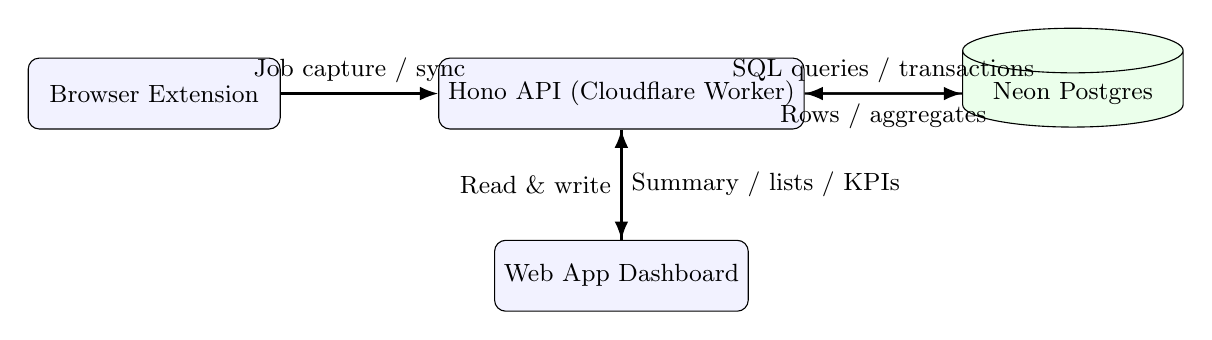
\begin{tikzpicture}[
  node distance=1.4cm and 2.0cm,
  every node/.style={font=\small},
  box/.style={draw, rounded corners, minimum width=3.2cm, minimum height=0.9cm, align=center, fill=blue!5},
  db/.style={draw, cylinder, shape border rotate=90, aspect=0.25, minimum height=1.0cm, minimum width=2.8cm, align=center, fill=green!8},
  edge/.style={-Latex, thick}
]
\node[box] (ext) {Browser Extension};
\node[box, right=of ext] (api) {Hono API (Cloudflare Worker)};
\node[db, right=of api] (db) {Neon Postgres};
\node[box, below=of api] (web) {Web App Dashboard};

\draw[edge] (ext) -- node[above]{Job capture / sync} (api);
\draw[edge] (web) -- node[left]{Read \& write} (api);
\draw[edge] (api) -- node[above]{SQL queries / transactions} (db);
\draw[edge] (db) -- node[below]{Rows / aggregates} (api);
\draw[edge] (api) -- node[right]{Summary / lists / KPIs} (web);
\end{tikzpicture}
\end{center}

\section{Entity Sync Matrix}
\begin{longtable}{p{0.20\linewidth}p{0.22\linewidth}p{0.23\linewidth}p{0.27\linewidth}}
\toprule
\textbf{Entity} & \textbf{Primary Writers} & \textbf{Primary Readers} & \textbf{Sync / Consistency Notes} \\
\midrule
\endfirsthead
\toprule
\textbf{Entity} & \textbf{Primary Writers} & \textbf{Primary Readers} & \textbf{Sync / Consistency Notes} \\
\midrule
\endhead
\texttt{dashboard\_users} & Auth signup/login/google, seed scripts & Auth middleware, social/network endpoints & \todoitem{Confirm unique constraints and update semantics.} \\
\texttt{dashboard\_sessions} & Session create/revoke & Auth middleware & \todoitem{Document TTL, revocation race handling, cleanup strategy.} \\
\texttt{jobs} & Jobs create/import/patch/delete, extension endpoint, seeds & Dashboard summary, jobs list/export, audits & \todoitem{Document dedupe strategy and idempotency guarantees.} \\
\texttt{referrals} & Referral CRUD + sync routines & Referral list/trends, dashboard summary & \todoitem{Document sync ownership and conflict resolution.} \\
\texttt{pending\_items} & Pending CRUD & Pending list and dashboard summary & \todoitem{Clarify archive semantics and dashboard visibility.} \\
\texttt{notes} & Notes CRUD & Notes list & \todoitem{Clarify retention and privacy scope.} \\
\texttt{friendships} & Friend request lifecycle & Friends/requests/network endpoints & \todoitem{Document lock ordering and status transitions.} \\
\texttt{user\_targets} & Target upsert endpoint & Target/progress and dashboard summaries & \todoitem{Confirm null/zero meaning by product requirements.} \\
\texttt{user\_field\_visibility} & Visibility patch endpoint & Network pages & \todoitem{Document required fields enforced by API.} \\
\bottomrule
\end{longtable}

\section{DB Call Inventory Summary}
\textbf{Total DB callsites discovered: 113}\\
\textbf{Source scope:} \texttt{UI interface/apps/api/src} and \texttt{UI interface/apps/api/scripts}

\begin{longtable}{p{0.10\linewidth}p{0.19\linewidth}p{0.10\linewidth}p{0.18\linewidth}p{0.16\linewidth}p{0.21\linewidth}}
\toprule
\textbf{ID} & \textbf{Context} & \textbf{Kind} & \textbf{Operation} & \textbf{Tables (detected)} & \textbf{Location} \\
\midrule
\endfirsthead
\toprule
\textbf{ID} & \textbf{Context} & \textbf{Kind} & \textbf{Operation} & \textbf{Tables (detected)} & \textbf{Location} \\
\midrule
\endhead
DB-001 & authMiddleware & query & SELECT & dashboard\_sessions, dashboard\_users & UI interface/apps/api/src/auth.ts:155 \\
DB-002 & createSession & query & INSERT & dashboard\_sessions & UI interface/apps/api/src/auth.ts:118 \\
DB-003 & DELETE /api/jobs/:id & query & DELETE & jobs, archive, online\_assessment\_records & UI interface/apps/api/src/index.ts:2955 \\
DB-004 & DELETE /api/notes/:id & query & DELETE & daily\_notes, pending\_items & UI interface/apps/api/src/index.ts:3777 \\
DB-005 & DELETE /api/oa/archive/:id & query & DELETE & online\_assessment\_records, referrals & UI interface/apps/api/src/index.ts:3489 \\
DB-006 & DELETE /api/referrals/:id & query & DELETE & referrals, daily\_notes & UI interface/apps/api/src/index.ts:3673 \\
DB-007 & ensureAcceptedFriendship & sql.query & INSERT & friendships, dashboard\_users & UI interface/apps/api/scripts/seed-network-demo-friends.js:214 \\
DB-008 & ensureOwnerUser & query & INSERT & dashboard\_users, dashboard\_sessions & UI interface/apps/api/src/auth.ts:100 \\
DB-009 & ensureOwnerUser & query & SELECT & dashboard\_users, dashboard\_sessions & UI interface/apps/api/src/auth.ts:105 \\
DB-010 & expectedJobsTrend & sql.query & SELECT & jobs & UI interface/apps/api/scripts/audit-dashboard-api.mjs:273 \\
DB-011 & expectedReferralsTrend & sql.query & SELECT & referrals, jobs & UI interface/apps/api/scripts/audit-dashboard-api.mjs:302 \\
DB-012 & expectedSummary & sql.query & SELECT & jobs, referrals, pending\_items & UI interface/apps/api/scripts/audit-dashboard-api.mjs:81 \\
DB-013 & expectedSummary & sql.query & SELECT & referrals, pending\_items, jobs & UI interface/apps/api/scripts/audit-dashboard-api.mjs:85 \\
DB-014 & expectedSummary & sql.query & SELECT & referrals, pending\_items, jobs & UI interface/apps/api/scripts/audit-dashboard-api.mjs:86 \\
DB-015 & expectedSummary & sql.query & SELECT & referrals, pending\_items, jobs & UI interface/apps/api/scripts/audit-dashboard-api.mjs:87 \\
DB-016 & expectedSummary & sql.query & SELECT & jobs & UI interface/apps/api/scripts/audit-dashboard-api.mjs:91 \\
DB-017 & expectedSummary & sql.query & SELECT & jobs & UI interface/apps/api/scripts/audit-dashboard-api.mjs:103 \\
DB-018 & expectedSummary & sql.query & SELECT & jobs & UI interface/apps/api/scripts/audit-dashboard-api.mjs:115 \\
DB-019 & expectedSummary & sql.query & SELECT & jobs & UI interface/apps/api/scripts/audit-dashboard-api.mjs:126 \\
DB-020 & expectedSummary & sql.query & SELECT & jobs & UI interface/apps/api/scripts/audit-dashboard-api.mjs:137 \\
DB-021 & expectedSummary & sql.query & SELECT & jobs & UI interface/apps/api/scripts/audit-dashboard-api.mjs:156 \\
DB-022 & expectedSummary & sql.query & SELECT & jobs, pending\_items & UI interface/apps/api/scripts/audit-dashboard-api.mjs:176 \\
DB-023 & expectedSummary & sql.query & SELECT & pending\_items, jobs & UI interface/apps/api/scripts/audit-dashboard-api.mjs:195 \\
DB-024 & expectedSummary & sql.query & WITH & jobs, weeks, counts & UI interface/apps/api/scripts/audit-dashboard-api.mjs:214 \\
DB-025 & expectedSummary & sql.query & SELECT & jobs & UI interface/apps/api/scripts/audit-dashboard-api.mjs:236 \\
DB-026 & firstLine & sql.query & DYNAMIC/UNKNOWN & TBD & UI interface/apps/api/scripts/run-migrations.js:92 \\
DB-027 & GET /api/dashboard/summary & query & SELECT & referrals, pending\_items, jobs & UI interface/apps/api/src/index.ts:1399 \\
DB-028 & GET /api/dashboard/summary & query & SELECT & referrals, pending\_items, jobs & UI interface/apps/api/src/index.ts:1400 \\
DB-029 & GET /api/dashboard/summary & query & SELECT & jobs & UI interface/apps/api/src/index.ts:1405 \\
DB-030 & GET /api/dashboard/summary & query & SELECT & jobs & UI interface/apps/api/src/index.ts:1417 \\
DB-031 & GET /api/dashboard/summary & query & SELECT & jobs & UI interface/apps/api/src/index.ts:1429 \\
DB-032 & GET /api/dashboard/summary & query & SELECT & jobs & UI interface/apps/api/src/index.ts:1440 \\
DB-033 & GET /api/dashboard/summary & query & SELECT & jobs & UI interface/apps/api/src/index.ts:1450 \\
DB-034 & GET /api/dashboard/summary & query & SELECT & jobs & UI interface/apps/api/src/index.ts:1456 \\
DB-035 & GET /api/dashboard/summary & query & SELECT & jobs & UI interface/apps/api/src/index.ts:1462 \\
DB-036 & GET /api/dashboard/summary & query & SELECT & jobs & UI interface/apps/api/src/index.ts:1485 \\
DB-037 & GET /api/dashboard/summary & query & SELECT & jobs & UI interface/apps/api/src/index.ts:1509 \\
DB-038 & GET /api/dashboard/summary & query & SELECT & pending\_items & UI interface/apps/api/src/index.ts:1533 \\
DB-039 & GET /api/dashboard/summary & query & SELECT & jobs & UI interface/apps/api/src/index.ts:1557 \\
DB-040 & GET /api/dashboard/summary & query & WITH & jobs, weeks, counts & UI interface/apps/api/src/index.ts:1584 \\
DB-041 & GET /api/dashboard/summary & query & SELECT & jobs & UI interface/apps/api/src/index.ts:1610 \\
DB-042 & GET /api/dashboard/summary & query & SELECT & jobs & UI interface/apps/api/src/index.ts:1623 \\
DB-043 & GET /api/dashboard/summary & query & SELECT & jobs & UI interface/apps/api/src/index.ts:1636 \\
DB-044 & GET /api/jobs & query & SELECT & jobs & UI interface/apps/api/src/index.ts:2348 \\
DB-045 & GET /api/jobs & query & DYNAMIC/UNKNOWN & TBD & UI interface/apps/api/src/index.ts:2358 \\
DB-046 & GET /api/jobs & query & SELECT & jobs & UI interface/apps/api/src/index.ts:2414 \\
DB-047 & GET /api/jobs & query & SELECT & jobs & UI interface/apps/api/src/index.ts:2431 \\
DB-048 & GET /api/jobs & query & INSERT & jobs & UI interface/apps/api/src/index.ts:2452 \\
DB-049 & GET /api/jobs/trend & query & SELECT & jobs & UI interface/apps/api/src/index.ts:1684 \\
DB-050 & GET /api/jobs/trend & query & SELECT & referrals & UI interface/apps/api/src/index.ts:2014 \\
DB-051 & GET /api/jobs/trend & query & SELECT & referrals & UI interface/apps/api/src/index.ts:2030 \\
DB-052 & GET /api/jobs/trend & query & UPDATE & referrals & UI interface/apps/api/src/index.ts:2051 \\
DB-053 & GET /api/jobs/trend & query & INSERT & referrals, jobs & UI interface/apps/api/src/index.ts:2084 \\
DB-054 & GET /api/notes & query & SELECT & daily\_notes & UI interface/apps/api/src/index.ts:3691 \\
DB-055 & GET /api/oa/active & query & WITH & archive, online\_assessment\_records, jobs, pending\_archive & UI interface/apps/api/src/index.ts:2970 \\
DB-056 & GET /api/oa/active & query & DELETE & online\_assessment\_records & UI interface/apps/api/src/index.ts:3006 \\
DB-057 & GET /api/oa/active & query & INSERT & online\_assessment\_records & UI interface/apps/api/src/index.ts:3017 \\
DB-058 & GET /api/pending & query & SELECT & pending\_items & UI interface/apps/api/src/index.ts:3791 \\
DB-059 & GET /api/pending & query & SELECT & pending\_items & UI interface/apps/api/src/index.ts:3797 \\
DB-060 & GET /api/referrals & query & SELECT & referrals & UI interface/apps/api/src/index.ts:3520 \\
DB-061 & GET /api/referrals/:id & query & SELECT & referrals & UI interface/apps/api/src/index.ts:3601 \\
DB-062 & GET /api/referrals/trend & query & WITH & referrals, jobs & UI interface/apps/api/src/index.ts:3560 \\
DB-063 & GET /api/targets/progress & query & SELECT & jobs & UI interface/apps/api/src/index.ts:513 \\
DB-064 & GET /api/targets/progress & query & SELECT & jobs & UI interface/apps/api/src/index.ts:525 \\
DB-065 & GET /api/targets/progress & query & SELECT & jobs & UI interface/apps/api/src/index.ts:538 \\
DB-066 & main & sql.query & WITH & jobs, candidate\_jobs, referrals & UI interface/apps/api/scripts/audit-referral-sync.js:54 \\
DB-067 & main & sql.query & WITH & jobs, candidate\_jobs, referrals & UI interface/apps/api/scripts/audit-referral-sync.js:87 \\
DB-068 & main & sql.query & WITH & jobs, candidate\_jobs, referrals & UI interface/apps/api/scripts/audit-referral-sync.js:131 \\
DB-069 & main & sql.query & WITH & jobs, candidate\_jobs, referrals & UI interface/apps/api/scripts/audit-referral-sync.js:170 \\
DB-070 & main & sql.query & SELECT & dashboard\_users & UI interface/apps/api/scripts/seed-network-demo-friends.js:241 \\
DB-071 & main & sql.query & INSERT & dashboard\_users, jobs & UI interface/apps/api/scripts/seed-network-demo-user.js:158 \\
DB-072 & main & sql.query & SELECT & dashboard\_users, jobs & UI interface/apps/api/scripts/seed-network-demo-user.js:171 \\
DB-073 & main & sql.query & DELETE & jobs & UI interface/apps/api/scripts/seed-network-demo-user.js:185 \\
DB-074 & main & sql.query & SELECT & dashboard\_users & UI interface/apps/api/scripts/seed-users.js:63 \\
DB-075 & main & sql.query & INSERT & dashboard\_users & UI interface/apps/api/scripts/seed-users.js:82 \\
DB-076 & main & sql.query & UPDATE & dashboard\_users & UI interface/apps/api/scripts/set-user-names.js:40 \\
DB-077 & main & sql.query & SELECT & dashboard\_users, completed & UI interface/apps/api/scripts/set-user-names.js:61 \\
DB-078 & main & sql.query & UPDATE & dashboard\_users, completed & UI interface/apps/api/scripts/set-user-names.js:77 \\
DB-079 & main & sql.query & WITH & jobs, referrals & UI interface/apps/api/scripts/sync-referrals-from-jobs.js:49 \\
DB-080 & PATCH /api/jobs/:id & query & UPDATE & jobs & UI interface/apps/api/src/index.ts:2904 \\
DB-081 & PATCH /api/notes/:id & query & UPDATE & daily\_notes, pending\_items & UI interface/apps/api/src/index.ts:3765 \\
DB-082 & PATCH /api/oa/archive/:id & query & DELETE & online\_assessment\_records & UI interface/apps/api/src/index.ts:3395 \\
DB-083 & PATCH /api/oa/archive/:id & query & UPDATE & online\_assessment\_records & UI interface/apps/api/src/index.ts:3477 \\
DB-084 & PATCH /api/pending/:id & query & UPDATE & pending\_items & UI interface/apps/api/src/index.ts:3886 \\
DB-085 & PATCH /api/referrals/:id & query & UPDATE & referrals & UI interface/apps/api/src/index.ts:3661 \\
DB-086 & POST /api/friends/:id/block & query & UPDATE & friendships & UI interface/apps/api/src/index.ts:873 \\
DB-087 & POST /api/friends/:id/reject & query & UPDATE & friendships & UI interface/apps/api/src/index.ts:846 \\
DB-088 & POST /api/friends/request & query & SELECT & dashboard\_users, friendships & UI interface/apps/api/src/index.ts:665 \\
DB-089 & POST /api/friends/request & query & SELECT & dashboard\_users, friendships & UI interface/apps/api/src/index.ts:674 \\
DB-090 & POST /api/friends/request & query & INSERT & friendships, incoming & UI interface/apps/api/src/index.ts:704 \\
DB-091 & POST /api/friends/request & query & UPDATE & friendships & UI interface/apps/api/src/index.ts:729 \\
DB-092 & POST /api/jobs/import/csv & transaction & SELECT & TBD & UI interface/apps/api/src/index.ts:2789 \\
DB-093 & POST /api/notes & query & INSERT & daily\_notes & UI interface/apps/api/src/index.ts:3717 \\
DB-094 & POST /api/oa/complete/:jobId & query & SELECT & online\_assessment\_records & UI interface/apps/api/src/index.ts:3153 \\
DB-095 & POST /api/pending & query & INSERT & pending\_items & UI interface/apps/api/src/index.ts:3819 \\
DB-096 & POST /api/referrals & query & INSERT & referrals, jobs & UI interface/apps/api/src/index.ts:3529 \\
DB-097 & POST /auth/google & query & SELECT & dashboard\_users & UI interface/apps/api/src/index.ts:345 \\
DB-098 & POST /auth/google & query & INSERT & dashboard\_users & UI interface/apps/api/src/index.ts:364 \\
DB-099 & POST /auth/google & query & UPDATE & dashboard\_users & UI interface/apps/api/src/index.ts:375 \\
DB-100 & POST /auth/signup & query & SELECT & dashboard\_users & UI interface/apps/api/src/index.ts:237 \\
DB-101 & POST /auth/signup & query & INSERT & dashboard\_users & UI interface/apps/api/src/index.ts:249 \\
DB-102 & query & sql.query & DYNAMIC/UNKNOWN & TBD & UI interface/apps/api/src/db.ts:17 \\
DB-103 & referralStatus & sql.query & INSERT & jobs & UI interface/apps/api/scripts/seed-network-demo-friends.js:91 \\
DB-104 & referralStatus & sql.query & INSERT & jobs & UI interface/apps/api/scripts/seed-network-demo-user.js:223 \\
DB-105 & resolveScopedUserId & sql.query & SELECT & dashboard\_users & UI interface/apps/api/scripts/audit-referral-sync.js:27 \\
DB-106 & resolveScopedUserId & sql.query & SELECT & dashboard\_users & UI interface/apps/api/scripts/sync-referrals-from-jobs.js:23 \\
DB-107 & revokeSession & query & UPDATE & dashboard\_sessions, dashboard\_users & UI interface/apps/api/src/auth.ts:131 \\
DB-108 & seedJobs & sql.query & DELETE & jobs & UI interface/apps/api/scripts/seed-network-demo-friends.js:82 \\
DB-109 & syncReferralsForUser & sql.query & WITH & jobs, referrals & UI interface/apps/api/scripts/seed-network-demo-friends.js:120 \\
DB-110 & syncReferralsForUser & sql.query & WITH & jobs, referrals & UI interface/apps/api/scripts/seed-network-demo-user.js:47 \\
DB-111 & transaction & sql.query & DYNAMIC/UNKNOWN & TBD & UI interface/apps/api/src/db.ts:32 \\
DB-112 & upsertUser & sql.query & INSERT & dashboard\_users, jobs & UI interface/apps/api/scripts/seed-network-demo-friends.js:65 \\
DB-113 & upsertUser & sql.query & SELECT & dashboard\_users, jobs & UI interface/apps/api/scripts/seed-network-demo-friends.js:77 \\
\bottomrule
\end{longtable}

\section{DB Calls A--Z (Detailed Template)}
\subsection{DB-001 - authMiddleware}
\begin{itemize}[leftmargin=1.5em]
\item \textbf{Location:} \texttt{UI interface/apps/api/src/auth.ts:155}
\item \textbf{Call kind:} \texttt{query}
\item \textbf{Detected operation:} \texttt{SELECT}
\item \textbf{Detected tables:} \texttt{dashboard\_sessions, dashboard\_users}
\item \textbf{Function context:} \texttt{authMiddleware}
\item \textbf{Code snippet:} \texttt{const [sessionUser] = await query<\{ id: number; email: string; first\_name: string | null; last\_name: string | null \}>(}
\item \textbf{Business purpose:} \todoitem{Describe why this query exists and expected behavior.}
\item \textbf{Inputs / params:} \todoitem{List each parameter, type, validation, and defaulting.}
\item \textbf{Output contract:} \todoitem{Define returned columns, shape, and nullability.}
\item \textbf{Failure modes:} \todoitem{DB errors, not-found behavior, conflict behavior, retries.}
\item \textbf{Security / tenancy:} \todoitem{Confirm user scoping and auth assumptions.}
\item \textbf{Performance:} \todoitem{Expected cardinality, index usage, and worst-case latency.}
\item \textbf{Sync impact:} \todoitem{Which downstream entities/views become stale; refresh rules.}
\item \textbf{Test coverage:} \todoitem{Unit/integration tests and missing cases.}
\item \textbf{Migration dependency:} \todoitem{Schema migration IDs required by this call.}
\end{itemize}
\subsection{DB-002 - createSession}
\begin{itemize}[leftmargin=1.5em]
\item \textbf{Location:} \texttt{UI interface/apps/api/src/auth.ts:118}
\item \textbf{Call kind:} \texttt{query}
\item \textbf{Detected operation:} \texttt{INSERT}
\item \textbf{Detected tables:} \texttt{dashboard\_sessions}
\item \textbf{Function context:} \texttt{createSession}
\item \textbf{Code snippet:} \texttt{await query(}
\item \textbf{Business purpose:} \todoitem{Describe why this query exists and expected behavior.}
\item \textbf{Inputs / params:} \todoitem{List each parameter, type, validation, and defaulting.}
\item \textbf{Output contract:} \todoitem{Define returned columns, shape, and nullability.}
\item \textbf{Failure modes:} \todoitem{DB errors, not-found behavior, conflict behavior, retries.}
\item \textbf{Security / tenancy:} \todoitem{Confirm user scoping and auth assumptions.}
\item \textbf{Performance:} \todoitem{Expected cardinality, index usage, and worst-case latency.}
\item \textbf{Sync impact:} \todoitem{Which downstream entities/views become stale; refresh rules.}
\item \textbf{Test coverage:} \todoitem{Unit/integration tests and missing cases.}
\item \textbf{Migration dependency:} \todoitem{Schema migration IDs required by this call.}
\end{itemize}
\subsection{DB-003 - DELETE /api/jobs/:id}
\begin{itemize}[leftmargin=1.5em]
\item \textbf{Location:} \texttt{UI interface/apps/api/src/index.ts:2955}
\item \textbf{Call kind:} \texttt{query}
\item \textbf{Detected operation:} \texttt{DELETE}
\item \textbf{Detected tables:} \texttt{jobs, archive, online\_assessment\_records}
\item \textbf{Function context:} \texttt{getCell}
\item \textbf{Code snippet:} \texttt{const rows = await query(}
\item \textbf{Business purpose:} \todoitem{Describe why this query exists and expected behavior.}
\item \textbf{Inputs / params:} \todoitem{List each parameter, type, validation, and defaulting.}
\item \textbf{Output contract:} \todoitem{Define returned columns, shape, and nullability.}
\item \textbf{Failure modes:} \todoitem{DB errors, not-found behavior, conflict behavior, retries.}
\item \textbf{Security / tenancy:} \todoitem{Confirm user scoping and auth assumptions.}
\item \textbf{Performance:} \todoitem{Expected cardinality, index usage, and worst-case latency.}
\item \textbf{Sync impact:} \todoitem{Which downstream entities/views become stale; refresh rules.}
\item \textbf{Test coverage:} \todoitem{Unit/integration tests and missing cases.}
\item \textbf{Migration dependency:} \todoitem{Schema migration IDs required by this call.}
\end{itemize}
\subsection{DB-004 - DELETE /api/notes/:id}
\begin{itemize}[leftmargin=1.5em]
\item \textbf{Location:} \texttt{UI interface/apps/api/src/index.ts:3777}
\item \textbf{Call kind:} \texttt{query}
\item \textbf{Detected operation:} \texttt{DELETE}
\item \textbf{Detected tables:} \texttt{daily\_notes, pending\_items}
\item \textbf{Function context:} \texttt{offset}
\item \textbf{Code snippet:} \texttt{const rows = await query(}
\item \textbf{Business purpose:} \todoitem{Describe why this query exists and expected behavior.}
\item \textbf{Inputs / params:} \todoitem{List each parameter, type, validation, and defaulting.}
\item \textbf{Output contract:} \todoitem{Define returned columns, shape, and nullability.}
\item \textbf{Failure modes:} \todoitem{DB errors, not-found behavior, conflict behavior, retries.}
\item \textbf{Security / tenancy:} \todoitem{Confirm user scoping and auth assumptions.}
\item \textbf{Performance:} \todoitem{Expected cardinality, index usage, and worst-case latency.}
\item \textbf{Sync impact:} \todoitem{Which downstream entities/views become stale; refresh rules.}
\item \textbf{Test coverage:} \todoitem{Unit/integration tests and missing cases.}
\item \textbf{Migration dependency:} \todoitem{Schema migration IDs required by this call.}
\end{itemize}
\subsection{DB-005 - DELETE /api/oa/archive/:id}
\begin{itemize}[leftmargin=1.5em]
\item \textbf{Location:} \texttt{UI interface/apps/api/src/index.ts:3489}
\item \textbf{Call kind:} \texttt{query}
\item \textbf{Detected operation:} \texttt{DELETE}
\item \textbf{Detected tables:} \texttt{online\_assessment\_records, referrals}
\item \textbf{Function context:} \texttt{getCell}
\item \textbf{Code snippet:} \texttt{const rows = await query(}
\item \textbf{Business purpose:} \todoitem{Describe why this query exists and expected behavior.}
\item \textbf{Inputs / params:} \todoitem{List each parameter, type, validation, and defaulting.}
\item \textbf{Output contract:} \todoitem{Define returned columns, shape, and nullability.}
\item \textbf{Failure modes:} \todoitem{DB errors, not-found behavior, conflict behavior, retries.}
\item \textbf{Security / tenancy:} \todoitem{Confirm user scoping and auth assumptions.}
\item \textbf{Performance:} \todoitem{Expected cardinality, index usage, and worst-case latency.}
\item \textbf{Sync impact:} \todoitem{Which downstream entities/views become stale; refresh rules.}
\item \textbf{Test coverage:} \todoitem{Unit/integration tests and missing cases.}
\item \textbf{Migration dependency:} \todoitem{Schema migration IDs required by this call.}
\end{itemize}
\subsection{DB-006 - DELETE /api/referrals/:id}
\begin{itemize}[leftmargin=1.5em]
\item \textbf{Location:} \texttt{UI interface/apps/api/src/index.ts:3673}
\item \textbf{Call kind:} \texttt{query}
\item \textbf{Detected operation:} \texttt{DELETE}
\item \textbf{Detected tables:} \texttt{referrals, daily\_notes}
\item \textbf{Function context:} \texttt{offset}
\item \textbf{Code snippet:} \texttt{const rows = await query(}
\item \textbf{Business purpose:} \todoitem{Describe why this query exists and expected behavior.}
\item \textbf{Inputs / params:} \todoitem{List each parameter, type, validation, and defaulting.}
\item \textbf{Output contract:} \todoitem{Define returned columns, shape, and nullability.}
\item \textbf{Failure modes:} \todoitem{DB errors, not-found behavior, conflict behavior, retries.}
\item \textbf{Security / tenancy:} \todoitem{Confirm user scoping and auth assumptions.}
\item \textbf{Performance:} \todoitem{Expected cardinality, index usage, and worst-case latency.}
\item \textbf{Sync impact:} \todoitem{Which downstream entities/views become stale; refresh rules.}
\item \textbf{Test coverage:} \todoitem{Unit/integration tests and missing cases.}
\item \textbf{Migration dependency:} \todoitem{Schema migration IDs required by this call.}
\end{itemize}
\subsection{DB-007 - ensureAcceptedFriendship}
\begin{itemize}[leftmargin=1.5em]
\item \textbf{Location:} \texttt{UI interface/apps/api/scripts/seed-network-demo-friends.js:214}
\item \textbf{Call kind:} \texttt{sql.query}
\item \textbf{Detected operation:} \texttt{INSERT}
\item \textbf{Detected tables:} \texttt{friendships, dashboard\_users}
\item \textbf{Function context:} \texttt{ensureAcceptedFriendship}
\item \textbf{Code snippet:} \texttt{await sql.query(}
\item \textbf{Business purpose:} \todoitem{Describe why this query exists and expected behavior.}
\item \textbf{Inputs / params:} \todoitem{List each parameter, type, validation, and defaulting.}
\item \textbf{Output contract:} \todoitem{Define returned columns, shape, and nullability.}
\item \textbf{Failure modes:} \todoitem{DB errors, not-found behavior, conflict behavior, retries.}
\item \textbf{Security / tenancy:} \todoitem{Confirm user scoping and auth assumptions.}
\item \textbf{Performance:} \todoitem{Expected cardinality, index usage, and worst-case latency.}
\item \textbf{Sync impact:} \todoitem{Which downstream entities/views become stale; refresh rules.}
\item \textbf{Test coverage:} \todoitem{Unit/integration tests and missing cases.}
\item \textbf{Migration dependency:} \todoitem{Schema migration IDs required by this call.}
\end{itemize}
\subsection{DB-008 - ensureOwnerUser}
\begin{itemize}[leftmargin=1.5em]
\item \textbf{Location:} \texttt{UI interface/apps/api/src/auth.ts:100}
\item \textbf{Call kind:} \texttt{query}
\item \textbf{Detected operation:} \texttt{INSERT}
\item \textbf{Detected tables:} \texttt{dashboard\_users, dashboard\_sessions}
\item \textbf{Function context:} \texttt{ensureOwnerUser}
\item \textbf{Code snippet:} \texttt{await query(}
\item \textbf{Business purpose:} \todoitem{Describe why this query exists and expected behavior.}
\item \textbf{Inputs / params:} \todoitem{List each parameter, type, validation, and defaulting.}
\item \textbf{Output contract:} \todoitem{Define returned columns, shape, and nullability.}
\item \textbf{Failure modes:} \todoitem{DB errors, not-found behavior, conflict behavior, retries.}
\item \textbf{Security / tenancy:} \todoitem{Confirm user scoping and auth assumptions.}
\item \textbf{Performance:} \todoitem{Expected cardinality, index usage, and worst-case latency.}
\item \textbf{Sync impact:} \todoitem{Which downstream entities/views become stale; refresh rules.}
\item \textbf{Test coverage:} \todoitem{Unit/integration tests and missing cases.}
\item \textbf{Migration dependency:} \todoitem{Schema migration IDs required by this call.}
\end{itemize}
\subsection{DB-009 - ensureOwnerUser}
\begin{itemize}[leftmargin=1.5em]
\item \textbf{Location:} \texttt{UI interface/apps/api/src/auth.ts:105}
\item \textbf{Call kind:} \texttt{query}
\item \textbf{Detected operation:} \texttt{SELECT}
\item \textbf{Detected tables:} \texttt{dashboard\_users, dashboard\_sessions}
\item \textbf{Function context:} \texttt{ensureOwnerUser}
\item \textbf{Code snippet:} \texttt{const [owner] = await query<\{ id: number; email: string; first\_name: string | null; last\_name: string | null \}>(}
\item \textbf{Business purpose:} \todoitem{Describe why this query exists and expected behavior.}
\item \textbf{Inputs / params:} \todoitem{List each parameter, type, validation, and defaulting.}
\item \textbf{Output contract:} \todoitem{Define returned columns, shape, and nullability.}
\item \textbf{Failure modes:} \todoitem{DB errors, not-found behavior, conflict behavior, retries.}
\item \textbf{Security / tenancy:} \todoitem{Confirm user scoping and auth assumptions.}
\item \textbf{Performance:} \todoitem{Expected cardinality, index usage, and worst-case latency.}
\item \textbf{Sync impact:} \todoitem{Which downstream entities/views become stale; refresh rules.}
\item \textbf{Test coverage:} \todoitem{Unit/integration tests and missing cases.}
\item \textbf{Migration dependency:} \todoitem{Schema migration IDs required by this call.}
\end{itemize}
\subsection{DB-010 - expectedJobsTrend}
\begin{itemize}[leftmargin=1.5em]
\item \textbf{Location:} \texttt{UI interface/apps/api/scripts/audit-dashboard-api.mjs:273}
\item \textbf{Call kind:} \texttt{sql.query}
\item \textbf{Detected operation:} \texttt{SELECT}
\item \textbf{Detected tables:} \texttt{jobs}
\item \textbf{Function context:} \texttt{expectedJobsTrend}
\item \textbf{Code snippet:} \texttt{return sql.query(}
\item \textbf{Business purpose:} \todoitem{Describe why this query exists and expected behavior.}
\item \textbf{Inputs / params:} \todoitem{List each parameter, type, validation, and defaulting.}
\item \textbf{Output contract:} \todoitem{Define returned columns, shape, and nullability.}
\item \textbf{Failure modes:} \todoitem{DB errors, not-found behavior, conflict behavior, retries.}
\item \textbf{Security / tenancy:} \todoitem{Confirm user scoping and auth assumptions.}
\item \textbf{Performance:} \todoitem{Expected cardinality, index usage, and worst-case latency.}
\item \textbf{Sync impact:} \todoitem{Which downstream entities/views become stale; refresh rules.}
\item \textbf{Test coverage:} \todoitem{Unit/integration tests and missing cases.}
\item \textbf{Migration dependency:} \todoitem{Schema migration IDs required by this call.}
\end{itemize}
\subsection{DB-011 - expectedReferralsTrend}
\begin{itemize}[leftmargin=1.5em]
\item \textbf{Location:} \texttt{UI interface/apps/api/scripts/audit-dashboard-api.mjs:302}
\item \textbf{Call kind:} \texttt{sql.query}
\item \textbf{Detected operation:} \texttt{SELECT}
\item \textbf{Detected tables:} \texttt{referrals, jobs}
\item \textbf{Function context:} \texttt{expectedReferralsTrend}
\item \textbf{Code snippet:} \texttt{return sql.query(}
\item \textbf{Business purpose:} \todoitem{Describe why this query exists and expected behavior.}
\item \textbf{Inputs / params:} \todoitem{List each parameter, type, validation, and defaulting.}
\item \textbf{Output contract:} \todoitem{Define returned columns, shape, and nullability.}
\item \textbf{Failure modes:} \todoitem{DB errors, not-found behavior, conflict behavior, retries.}
\item \textbf{Security / tenancy:} \todoitem{Confirm user scoping and auth assumptions.}
\item \textbf{Performance:} \todoitem{Expected cardinality, index usage, and worst-case latency.}
\item \textbf{Sync impact:} \todoitem{Which downstream entities/views become stale; refresh rules.}
\item \textbf{Test coverage:} \todoitem{Unit/integration tests and missing cases.}
\item \textbf{Migration dependency:} \todoitem{Schema migration IDs required by this call.}
\end{itemize}
\subsection{DB-012 - expectedSummary}
\begin{itemize}[leftmargin=1.5em]
\item \textbf{Location:} \texttt{UI interface/apps/api/scripts/audit-dashboard-api.mjs:81}
\item \textbf{Call kind:} \texttt{sql.query}
\item \textbf{Detected operation:} \texttt{SELECT}
\item \textbf{Detected tables:} \texttt{jobs, referrals, pending\_items}
\item \textbf{Function context:} \texttt{expectedSummary}
\item \textbf{Code snippet:} \texttt{const [jobs] = await sql.query(}
\item \textbf{Business purpose:} \todoitem{Describe why this query exists and expected behavior.}
\item \textbf{Inputs / params:} \todoitem{List each parameter, type, validation, and defaulting.}
\item \textbf{Output contract:} \todoitem{Define returned columns, shape, and nullability.}
\item \textbf{Failure modes:} \todoitem{DB errors, not-found behavior, conflict behavior, retries.}
\item \textbf{Security / tenancy:} \todoitem{Confirm user scoping and auth assumptions.}
\item \textbf{Performance:} \todoitem{Expected cardinality, index usage, and worst-case latency.}
\item \textbf{Sync impact:} \todoitem{Which downstream entities/views become stale; refresh rules.}
\item \textbf{Test coverage:} \todoitem{Unit/integration tests and missing cases.}
\item \textbf{Migration dependency:} \todoitem{Schema migration IDs required by this call.}
\end{itemize}
\subsection{DB-013 - expectedSummary}
\begin{itemize}[leftmargin=1.5em]
\item \textbf{Location:} \texttt{UI interface/apps/api/scripts/audit-dashboard-api.mjs:85}
\item \textbf{Call kind:} \texttt{sql.query}
\item \textbf{Detected operation:} \texttt{SELECT}
\item \textbf{Detected tables:} \texttt{referrals, pending\_items, jobs}
\item \textbf{Function context:} \texttt{expectedSummary}
\item \textbf{Code snippet:} \texttt{const [referrals] = await sql.query("SELECT COUNT(*)::int AS c FROM referrals WHERE user\_id = \$1", [userId]);}
\item \textbf{Business purpose:} \todoitem{Describe why this query exists and expected behavior.}
\item \textbf{Inputs / params:} \todoitem{List each parameter, type, validation, and defaulting.}
\item \textbf{Output contract:} \todoitem{Define returned columns, shape, and nullability.}
\item \textbf{Failure modes:} \todoitem{DB errors, not-found behavior, conflict behavior, retries.}
\item \textbf{Security / tenancy:} \todoitem{Confirm user scoping and auth assumptions.}
\item \textbf{Performance:} \todoitem{Expected cardinality, index usage, and worst-case latency.}
\item \textbf{Sync impact:} \todoitem{Which downstream entities/views become stale; refresh rules.}
\item \textbf{Test coverage:} \todoitem{Unit/integration tests and missing cases.}
\item \textbf{Migration dependency:} \todoitem{Schema migration IDs required by this call.}
\end{itemize}
\subsection{DB-014 - expectedSummary}
\begin{itemize}[leftmargin=1.5em]
\item \textbf{Location:} \texttt{UI interface/apps/api/scripts/audit-dashboard-api.mjs:86}
\item \textbf{Call kind:} \texttt{sql.query}
\item \textbf{Detected operation:} \texttt{SELECT}
\item \textbf{Detected tables:} \texttt{referrals, pending\_items, jobs}
\item \textbf{Function context:} \texttt{expectedSummary}
\item \textbf{Code snippet:} \texttt{const [pending] = await sql.query("SELECT COUNT(*)::int AS c FROM pending\_items WHERE user\_id = \$1 AND is\_done = FALSE", [userId]);}
\item \textbf{Business purpose:} \todoitem{Describe why this query exists and expected behavior.}
\item \textbf{Inputs / params:} \todoitem{List each parameter, type, validation, and defaulting.}
\item \textbf{Output contract:} \todoitem{Define returned columns, shape, and nullability.}
\item \textbf{Failure modes:} \todoitem{DB errors, not-found behavior, conflict behavior, retries.}
\item \textbf{Security / tenancy:} \todoitem{Confirm user scoping and auth assumptions.}
\item \textbf{Performance:} \todoitem{Expected cardinality, index usage, and worst-case latency.}
\item \textbf{Sync impact:} \todoitem{Which downstream entities/views become stale; refresh rules.}
\item \textbf{Test coverage:} \todoitem{Unit/integration tests and missing cases.}
\item \textbf{Migration dependency:} \todoitem{Schema migration IDs required by this call.}
\end{itemize}
\subsection{DB-015 - expectedSummary}
\begin{itemize}[leftmargin=1.5em]
\item \textbf{Location:} \texttt{UI interface/apps/api/scripts/audit-dashboard-api.mjs:87}
\item \textbf{Call kind:} \texttt{sql.query}
\item \textbf{Detected operation:} \texttt{SELECT}
\item \textbf{Detected tables:} \texttt{referrals, pending\_items, jobs}
\item \textbf{Function context:} \texttt{expectedSummary}
\item \textbf{Code snippet:} \texttt{const [rejected] = await sql.query(}
\item \textbf{Business purpose:} \todoitem{Describe why this query exists and expected behavior.}
\item \textbf{Inputs / params:} \todoitem{List each parameter, type, validation, and defaulting.}
\item \textbf{Output contract:} \todoitem{Define returned columns, shape, and nullability.}
\item \textbf{Failure modes:} \todoitem{DB errors, not-found behavior, conflict behavior, retries.}
\item \textbf{Security / tenancy:} \todoitem{Confirm user scoping and auth assumptions.}
\item \textbf{Performance:} \todoitem{Expected cardinality, index usage, and worst-case latency.}
\item \textbf{Sync impact:} \todoitem{Which downstream entities/views become stale; refresh rules.}
\item \textbf{Test coverage:} \todoitem{Unit/integration tests and missing cases.}
\item \textbf{Migration dependency:} \todoitem{Schema migration IDs required by this call.}
\end{itemize}
\subsection{DB-016 - expectedSummary}
\begin{itemize}[leftmargin=1.5em]
\item \textbf{Location:} \texttt{UI interface/apps/api/scripts/audit-dashboard-api.mjs:91}
\item \textbf{Call kind:} \texttt{sql.query}
\item \textbf{Detected operation:} \texttt{SELECT}
\item \textbf{Detected tables:} \texttt{jobs}
\item \textbf{Function context:} \texttt{expectedSummary}
\item \textbf{Code snippet:} \texttt{const [jobsThisMonth] = await sql.query(}
\item \textbf{Business purpose:} \todoitem{Describe why this query exists and expected behavior.}
\item \textbf{Inputs / params:} \todoitem{List each parameter, type, validation, and defaulting.}
\item \textbf{Output contract:} \todoitem{Define returned columns, shape, and nullability.}
\item \textbf{Failure modes:} \todoitem{DB errors, not-found behavior, conflict behavior, retries.}
\item \textbf{Security / tenancy:} \todoitem{Confirm user scoping and auth assumptions.}
\item \textbf{Performance:} \todoitem{Expected cardinality, index usage, and worst-case latency.}
\item \textbf{Sync impact:} \todoitem{Which downstream entities/views become stale; refresh rules.}
\item \textbf{Test coverage:} \todoitem{Unit/integration tests and missing cases.}
\item \textbf{Migration dependency:} \todoitem{Schema migration IDs required by this call.}
\end{itemize}
\subsection{DB-017 - expectedSummary}
\begin{itemize}[leftmargin=1.5em]
\item \textbf{Location:} \texttt{UI interface/apps/api/scripts/audit-dashboard-api.mjs:103}
\item \textbf{Call kind:} \texttt{sql.query}
\item \textbf{Detected operation:} \texttt{SELECT}
\item \textbf{Detected tables:} \texttt{jobs}
\item \textbf{Function context:} \texttt{expectedSummary}
\item \textbf{Code snippet:} \texttt{const [jobsThisWeek] = await sql.query(}
\item \textbf{Business purpose:} \todoitem{Describe why this query exists and expected behavior.}
\item \textbf{Inputs / params:} \todoitem{List each parameter, type, validation, and defaulting.}
\item \textbf{Output contract:} \todoitem{Define returned columns, shape, and nullability.}
\item \textbf{Failure modes:} \todoitem{DB errors, not-found behavior, conflict behavior, retries.}
\item \textbf{Security / tenancy:} \todoitem{Confirm user scoping and auth assumptions.}
\item \textbf{Performance:} \todoitem{Expected cardinality, index usage, and worst-case latency.}
\item \textbf{Sync impact:} \todoitem{Which downstream entities/views become stale; refresh rules.}
\item \textbf{Test coverage:} \todoitem{Unit/integration tests and missing cases.}
\item \textbf{Migration dependency:} \todoitem{Schema migration IDs required by this call.}
\end{itemize}
\subsection{DB-018 - expectedSummary}
\begin{itemize}[leftmargin=1.5em]
\item \textbf{Location:} \texttt{UI interface/apps/api/scripts/audit-dashboard-api.mjs:115}
\item \textbf{Call kind:} \texttt{sql.query}
\item \textbf{Detected operation:} \texttt{SELECT}
\item \textbf{Detected tables:} \texttt{jobs}
\item \textbf{Function context:} \texttt{expectedSummary}
\item \textbf{Code snippet:} \texttt{const [jobsToday] = await sql.query(}
\item \textbf{Business purpose:} \todoitem{Describe why this query exists and expected behavior.}
\item \textbf{Inputs / params:} \todoitem{List each parameter, type, validation, and defaulting.}
\item \textbf{Output contract:} \todoitem{Define returned columns, shape, and nullability.}
\item \textbf{Failure modes:} \todoitem{DB errors, not-found behavior, conflict behavior, retries.}
\item \textbf{Security / tenancy:} \todoitem{Confirm user scoping and auth assumptions.}
\item \textbf{Performance:} \todoitem{Expected cardinality, index usage, and worst-case latency.}
\item \textbf{Sync impact:} \todoitem{Which downstream entities/views become stale; refresh rules.}
\item \textbf{Test coverage:} \todoitem{Unit/integration tests and missing cases.}
\item \textbf{Migration dependency:} \todoitem{Schema migration IDs required by this call.}
\end{itemize}
\subsection{DB-019 - expectedSummary}
\begin{itemize}[leftmargin=1.5em]
\item \textbf{Location:} \texttt{UI interface/apps/api/scripts/audit-dashboard-api.mjs:126}
\item \textbf{Call kind:} \texttt{sql.query}
\item \textbf{Detected operation:} \texttt{SELECT}
\item \textbf{Detected tables:} \texttt{jobs}
\item \textbf{Function context:} \texttt{expectedSummary}
\item \textbf{Code snippet:} \texttt{const [jobsWithReferral] = await sql.query(}
\item \textbf{Business purpose:} \todoitem{Describe why this query exists and expected behavior.}
\item \textbf{Inputs / params:} \todoitem{List each parameter, type, validation, and defaulting.}
\item \textbf{Output contract:} \todoitem{Define returned columns, shape, and nullability.}
\item \textbf{Failure modes:} \todoitem{DB errors, not-found behavior, conflict behavior, retries.}
\item \textbf{Security / tenancy:} \todoitem{Confirm user scoping and auth assumptions.}
\item \textbf{Performance:} \todoitem{Expected cardinality, index usage, and worst-case latency.}
\item \textbf{Sync impact:} \todoitem{Which downstream entities/views become stale; refresh rules.}
\item \textbf{Test coverage:} \todoitem{Unit/integration tests and missing cases.}
\item \textbf{Migration dependency:} \todoitem{Schema migration IDs required by this call.}
\end{itemize}
\subsection{DB-020 - expectedSummary}
\begin{itemize}[leftmargin=1.5em]
\item \textbf{Location:} \texttt{UI interface/apps/api/scripts/audit-dashboard-api.mjs:137}
\item \textbf{Call kind:} \texttt{sql.query}
\item \textbf{Detected operation:} \texttt{SELECT}
\item \textbf{Detected tables:} \texttt{jobs}
\item \textbf{Function context:} \texttt{expectedSummary}
\item \textbf{Code snippet:} \texttt{const dailyTrend = await sql.query(}
\item \textbf{Business purpose:} \todoitem{Describe why this query exists and expected behavior.}
\item \textbf{Inputs / params:} \todoitem{List each parameter, type, validation, and defaulting.}
\item \textbf{Output contract:} \todoitem{Define returned columns, shape, and nullability.}
\item \textbf{Failure modes:} \todoitem{DB errors, not-found behavior, conflict behavior, retries.}
\item \textbf{Security / tenancy:} \todoitem{Confirm user scoping and auth assumptions.}
\item \textbf{Performance:} \todoitem{Expected cardinality, index usage, and worst-case latency.}
\item \textbf{Sync impact:} \todoitem{Which downstream entities/views become stale; refresh rules.}
\item \textbf{Test coverage:} \todoitem{Unit/integration tests and missing cases.}
\item \textbf{Migration dependency:} \todoitem{Schema migration IDs required by this call.}
\end{itemize}
\subsection{DB-021 - expectedSummary}
\begin{itemize}[leftmargin=1.5em]
\item \textbf{Location:} \texttt{UI interface/apps/api/scripts/audit-dashboard-api.mjs:156}
\item \textbf{Call kind:} \texttt{sql.query}
\item \textbf{Detected operation:} \texttt{SELECT}
\item \textbf{Detected tables:} \texttt{jobs}
\item \textbf{Function context:} \texttt{expectedSummary}
\item \textbf{Code snippet:} \texttt{const referralDailyTrend = await sql.query(}
\item \textbf{Business purpose:} \todoitem{Describe why this query exists and expected behavior.}
\item \textbf{Inputs / params:} \todoitem{List each parameter, type, validation, and defaulting.}
\item \textbf{Output contract:} \todoitem{Define returned columns, shape, and nullability.}
\item \textbf{Failure modes:} \todoitem{DB errors, not-found behavior, conflict behavior, retries.}
\item \textbf{Security / tenancy:} \todoitem{Confirm user scoping and auth assumptions.}
\item \textbf{Performance:} \todoitem{Expected cardinality, index usage, and worst-case latency.}
\item \textbf{Sync impact:} \todoitem{Which downstream entities/views become stale; refresh rules.}
\item \textbf{Test coverage:} \todoitem{Unit/integration tests and missing cases.}
\item \textbf{Migration dependency:} \todoitem{Schema migration IDs required by this call.}
\end{itemize}
\subsection{DB-022 - expectedSummary}
\begin{itemize}[leftmargin=1.5em]
\item \textbf{Location:} \texttt{UI interface/apps/api/scripts/audit-dashboard-api.mjs:176}
\item \textbf{Call kind:} \texttt{sql.query}
\item \textbf{Detected operation:} \texttt{SELECT}
\item \textbf{Detected tables:} \texttt{jobs, pending\_items}
\item \textbf{Function context:} \texttt{expectedSummary}
\item \textbf{Code snippet:} \texttt{const rejectedDailyTrend = await sql.query(}
\item \textbf{Business purpose:} \todoitem{Describe why this query exists and expected behavior.}
\item \textbf{Inputs / params:} \todoitem{List each parameter, type, validation, and defaulting.}
\item \textbf{Output contract:} \todoitem{Define returned columns, shape, and nullability.}
\item \textbf{Failure modes:} \todoitem{DB errors, not-found behavior, conflict behavior, retries.}
\item \textbf{Security / tenancy:} \todoitem{Confirm user scoping and auth assumptions.}
\item \textbf{Performance:} \todoitem{Expected cardinality, index usage, and worst-case latency.}
\item \textbf{Sync impact:} \todoitem{Which downstream entities/views become stale; refresh rules.}
\item \textbf{Test coverage:} \todoitem{Unit/integration tests and missing cases.}
\item \textbf{Migration dependency:} \todoitem{Schema migration IDs required by this call.}
\end{itemize}
\subsection{DB-023 - expectedSummary}
\begin{itemize}[leftmargin=1.5em]
\item \textbf{Location:} \texttt{UI interface/apps/api/scripts/audit-dashboard-api.mjs:195}
\item \textbf{Call kind:} \texttt{sql.query}
\item \textbf{Detected operation:} \texttt{SELECT}
\item \textbf{Detected tables:} \texttt{pending\_items, jobs}
\item \textbf{Function context:} \texttt{expectedSummary}
\item \textbf{Code snippet:} \texttt{const pendingDailyTrend = await sql.query(}
\item \textbf{Business purpose:} \todoitem{Describe why this query exists and expected behavior.}
\item \textbf{Inputs / params:} \todoitem{List each parameter, type, validation, and defaulting.}
\item \textbf{Output contract:} \todoitem{Define returned columns, shape, and nullability.}
\item \textbf{Failure modes:} \todoitem{DB errors, not-found behavior, conflict behavior, retries.}
\item \textbf{Security / tenancy:} \todoitem{Confirm user scoping and auth assumptions.}
\item \textbf{Performance:} \todoitem{Expected cardinality, index usage, and worst-case latency.}
\item \textbf{Sync impact:} \todoitem{Which downstream entities/views become stale; refresh rules.}
\item \textbf{Test coverage:} \todoitem{Unit/integration tests and missing cases.}
\item \textbf{Migration dependency:} \todoitem{Schema migration IDs required by this call.}
\end{itemize}
\subsection{DB-024 - expectedSummary}
\begin{itemize}[leftmargin=1.5em]
\item \textbf{Location:} \texttt{UI interface/apps/api/scripts/audit-dashboard-api.mjs:214}
\item \textbf{Call kind:} \texttt{sql.query}
\item \textbf{Detected operation:} \texttt{WITH}
\item \textbf{Detected tables:} \texttt{jobs, weeks, counts}
\item \textbf{Function context:} \texttt{expectedSummary}
\item \textbf{Code snippet:} \texttt{const weeklyTrend = await sql.query(}
\item \textbf{Business purpose:} \todoitem{Describe why this query exists and expected behavior.}
\item \textbf{Inputs / params:} \todoitem{List each parameter, type, validation, and defaulting.}
\item \textbf{Output contract:} \todoitem{Define returned columns, shape, and nullability.}
\item \textbf{Failure modes:} \todoitem{DB errors, not-found behavior, conflict behavior, retries.}
\item \textbf{Security / tenancy:} \todoitem{Confirm user scoping and auth assumptions.}
\item \textbf{Performance:} \todoitem{Expected cardinality, index usage, and worst-case latency.}
\item \textbf{Sync impact:} \todoitem{Which downstream entities/views become stale; refresh rules.}
\item \textbf{Test coverage:} \todoitem{Unit/integration tests and missing cases.}
\item \textbf{Migration dependency:} \todoitem{Schema migration IDs required by this call.}
\end{itemize}
\subsection{DB-025 - expectedSummary}
\begin{itemize}[leftmargin=1.5em]
\item \textbf{Location:} \texttt{UI interface/apps/api/scripts/audit-dashboard-api.mjs:236}
\item \textbf{Call kind:} \texttt{sql.query}
\item \textbf{Detected operation:} \texttt{SELECT}
\item \textbf{Detected tables:} \texttt{jobs}
\item \textbf{Function context:} \texttt{expectedSummary}
\item \textbf{Code snippet:} \texttt{const monthlyTrend = await sql.query(}
\item \textbf{Business purpose:} \todoitem{Describe why this query exists and expected behavior.}
\item \textbf{Inputs / params:} \todoitem{List each parameter, type, validation, and defaulting.}
\item \textbf{Output contract:} \todoitem{Define returned columns, shape, and nullability.}
\item \textbf{Failure modes:} \todoitem{DB errors, not-found behavior, conflict behavior, retries.}
\item \textbf{Security / tenancy:} \todoitem{Confirm user scoping and auth assumptions.}
\item \textbf{Performance:} \todoitem{Expected cardinality, index usage, and worst-case latency.}
\item \textbf{Sync impact:} \todoitem{Which downstream entities/views become stale; refresh rules.}
\item \textbf{Test coverage:} \todoitem{Unit/integration tests and missing cases.}
\item \textbf{Migration dependency:} \todoitem{Schema migration IDs required by this call.}
\end{itemize}
\subsection{DB-026 - firstLine}
\begin{itemize}[leftmargin=1.5em]
\item \textbf{Location:} \texttt{UI interface/apps/api/scripts/run-migrations.js:92}
\item \textbf{Call kind:} \texttt{sql.query}
\item \textbf{Detected operation:} \texttt{DYNAMIC/UNKNOWN}
\item \textbf{Detected tables:} \texttt{TBD}
\item \textbf{Function context:} \texttt{firstLine}
\item \textbf{Code snippet:} \texttt{if (statement) await sql.query(statement + ";", []);}
\item \textbf{Business purpose:} \todoitem{Describe why this query exists and expected behavior.}
\item \textbf{Inputs / params:} \todoitem{List each parameter, type, validation, and defaulting.}
\item \textbf{Output contract:} \todoitem{Define returned columns, shape, and nullability.}
\item \textbf{Failure modes:} \todoitem{DB errors, not-found behavior, conflict behavior, retries.}
\item \textbf{Security / tenancy:} \todoitem{Confirm user scoping and auth assumptions.}
\item \textbf{Performance:} \todoitem{Expected cardinality, index usage, and worst-case latency.}
\item \textbf{Sync impact:} \todoitem{Which downstream entities/views become stale; refresh rules.}
\item \textbf{Test coverage:} \todoitem{Unit/integration tests and missing cases.}
\item \textbf{Migration dependency:} \todoitem{Schema migration IDs required by this call.}
\end{itemize}
\subsection{DB-027 - GET /api/dashboard/summary}
\begin{itemize}[leftmargin=1.5em]
\item \textbf{Location:} \texttt{UI interface/apps/api/src/index.ts:1399}
\item \textbf{Call kind:} \texttt{query}
\item \textbf{Detected operation:} \texttt{SELECT}
\item \textbf{Detected tables:} \texttt{referrals, pending\_items, jobs}
\item \textbf{Function context:} \texttt{verifyGoogleIdToken}
\item \textbf{Code snippet:} \texttt{const [referralCount] = await query<\{ count: string \}>(env, "SELECT COUNT(*)::text AS count FROM referrals WHERE user\_id = \$1", [userId]);}
\item \textbf{Business purpose:} \todoitem{Describe why this query exists and expected behavior.}
\item \textbf{Inputs / params:} \todoitem{List each parameter, type, validation, and defaulting.}
\item \textbf{Output contract:} \todoitem{Define returned columns, shape, and nullability.}
\item \textbf{Failure modes:} \todoitem{DB errors, not-found behavior, conflict behavior, retries.}
\item \textbf{Security / tenancy:} \todoitem{Confirm user scoping and auth assumptions.}
\item \textbf{Performance:} \todoitem{Expected cardinality, index usage, and worst-case latency.}
\item \textbf{Sync impact:} \todoitem{Which downstream entities/views become stale; refresh rules.}
\item \textbf{Test coverage:} \todoitem{Unit/integration tests and missing cases.}
\item \textbf{Migration dependency:} \todoitem{Schema migration IDs required by this call.}
\end{itemize}
\subsection{DB-028 - GET /api/dashboard/summary}
\begin{itemize}[leftmargin=1.5em]
\item \textbf{Location:} \texttt{UI interface/apps/api/src/index.ts:1400}
\item \textbf{Call kind:} \texttt{query}
\item \textbf{Detected operation:} \texttt{SELECT}
\item \textbf{Detected tables:} \texttt{referrals, pending\_items, jobs}
\item \textbf{Function context:} \texttt{verifyGoogleIdToken}
\item \textbf{Code snippet:} \texttt{const [pendingCount] = await query<\{ count: string \}>(}
\item \textbf{Business purpose:} \todoitem{Describe why this query exists and expected behavior.}
\item \textbf{Inputs / params:} \todoitem{List each parameter, type, validation, and defaulting.}
\item \textbf{Output contract:} \todoitem{Define returned columns, shape, and nullability.}
\item \textbf{Failure modes:} \todoitem{DB errors, not-found behavior, conflict behavior, retries.}
\item \textbf{Security / tenancy:} \todoitem{Confirm user scoping and auth assumptions.}
\item \textbf{Performance:} \todoitem{Expected cardinality, index usage, and worst-case latency.}
\item \textbf{Sync impact:} \todoitem{Which downstream entities/views become stale; refresh rules.}
\item \textbf{Test coverage:} \todoitem{Unit/integration tests and missing cases.}
\item \textbf{Migration dependency:} \todoitem{Schema migration IDs required by this call.}
\end{itemize}
\subsection{DB-029 - GET /api/dashboard/summary}
\begin{itemize}[leftmargin=1.5em]
\item \textbf{Location:} \texttt{UI interface/apps/api/src/index.ts:1405}
\item \textbf{Call kind:} \texttt{query}
\item \textbf{Detected operation:} \texttt{SELECT}
\item \textbf{Detected tables:} \texttt{jobs}
\item \textbf{Function context:} \texttt{verifyGoogleIdToken}
\item \textbf{Code snippet:} \texttt{const [jobsThisMonth] = await query<\{ count: string \}>(}
\item \textbf{Business purpose:} \todoitem{Describe why this query exists and expected behavior.}
\item \textbf{Inputs / params:} \todoitem{List each parameter, type, validation, and defaulting.}
\item \textbf{Output contract:} \todoitem{Define returned columns, shape, and nullability.}
\item \textbf{Failure modes:} \todoitem{DB errors, not-found behavior, conflict behavior, retries.}
\item \textbf{Security / tenancy:} \todoitem{Confirm user scoping and auth assumptions.}
\item \textbf{Performance:} \todoitem{Expected cardinality, index usage, and worst-case latency.}
\item \textbf{Sync impact:} \todoitem{Which downstream entities/views become stale; refresh rules.}
\item \textbf{Test coverage:} \todoitem{Unit/integration tests and missing cases.}
\item \textbf{Migration dependency:} \todoitem{Schema migration IDs required by this call.}
\end{itemize}
\subsection{DB-030 - GET /api/dashboard/summary}
\begin{itemize}[leftmargin=1.5em]
\item \textbf{Location:} \texttt{UI interface/apps/api/src/index.ts:1417}
\item \textbf{Call kind:} \texttt{query}
\item \textbf{Detected operation:} \texttt{SELECT}
\item \textbf{Detected tables:} \texttt{jobs}
\item \textbf{Function context:} \texttt{verifyGoogleIdToken}
\item \textbf{Code snippet:} \texttt{const [jobsThisWeek] = await query<\{ count: string \}>(}
\item \textbf{Business purpose:} \todoitem{Describe why this query exists and expected behavior.}
\item \textbf{Inputs / params:} \todoitem{List each parameter, type, validation, and defaulting.}
\item \textbf{Output contract:} \todoitem{Define returned columns, shape, and nullability.}
\item \textbf{Failure modes:} \todoitem{DB errors, not-found behavior, conflict behavior, retries.}
\item \textbf{Security / tenancy:} \todoitem{Confirm user scoping and auth assumptions.}
\item \textbf{Performance:} \todoitem{Expected cardinality, index usage, and worst-case latency.}
\item \textbf{Sync impact:} \todoitem{Which downstream entities/views become stale; refresh rules.}
\item \textbf{Test coverage:} \todoitem{Unit/integration tests and missing cases.}
\item \textbf{Migration dependency:} \todoitem{Schema migration IDs required by this call.}
\end{itemize}
\subsection{DB-031 - GET /api/dashboard/summary}
\begin{itemize}[leftmargin=1.5em]
\item \textbf{Location:} \texttt{UI interface/apps/api/src/index.ts:1429}
\item \textbf{Call kind:} \texttt{query}
\item \textbf{Detected operation:} \texttt{SELECT}
\item \textbf{Detected tables:} \texttt{jobs}
\item \textbf{Function context:} \texttt{verifyGoogleIdToken}
\item \textbf{Code snippet:} \texttt{const [jobsToday] = await query<\{ count: string \}>(}
\item \textbf{Business purpose:} \todoitem{Describe why this query exists and expected behavior.}
\item \textbf{Inputs / params:} \todoitem{List each parameter, type, validation, and defaulting.}
\item \textbf{Output contract:} \todoitem{Define returned columns, shape, and nullability.}
\item \textbf{Failure modes:} \todoitem{DB errors, not-found behavior, conflict behavior, retries.}
\item \textbf{Security / tenancy:} \todoitem{Confirm user scoping and auth assumptions.}
\item \textbf{Performance:} \todoitem{Expected cardinality, index usage, and worst-case latency.}
\item \textbf{Sync impact:} \todoitem{Which downstream entities/views become stale; refresh rules.}
\item \textbf{Test coverage:} \todoitem{Unit/integration tests and missing cases.}
\item \textbf{Migration dependency:} \todoitem{Schema migration IDs required by this call.}
\end{itemize}
\subsection{DB-032 - GET /api/dashboard/summary}
\begin{itemize}[leftmargin=1.5em]
\item \textbf{Location:} \texttt{UI interface/apps/api/src/index.ts:1440}
\item \textbf{Call kind:} \texttt{query}
\item \textbf{Detected operation:} \texttt{SELECT}
\item \textbf{Detected tables:} \texttt{jobs}
\item \textbf{Function context:} \texttt{verifyGoogleIdToken}
\item \textbf{Code snippet:} \texttt{const [jobsWithReferral] = await query<\{ count: string \}>(}
\item \textbf{Business purpose:} \todoitem{Describe why this query exists and expected behavior.}
\item \textbf{Inputs / params:} \todoitem{List each parameter, type, validation, and defaulting.}
\item \textbf{Output contract:} \todoitem{Define returned columns, shape, and nullability.}
\item \textbf{Failure modes:} \todoitem{DB errors, not-found behavior, conflict behavior, retries.}
\item \textbf{Security / tenancy:} \todoitem{Confirm user scoping and auth assumptions.}
\item \textbf{Performance:} \todoitem{Expected cardinality, index usage, and worst-case latency.}
\item \textbf{Sync impact:} \todoitem{Which downstream entities/views become stale; refresh rules.}
\item \textbf{Test coverage:} \todoitem{Unit/integration tests and missing cases.}
\item \textbf{Migration dependency:} \todoitem{Schema migration IDs required by this call.}
\end{itemize}
\subsection{DB-033 - GET /api/dashboard/summary}
\begin{itemize}[leftmargin=1.5em]
\item \textbf{Location:} \texttt{UI interface/apps/api/src/index.ts:1450}
\item \textbf{Call kind:} \texttt{query}
\item \textbf{Detected operation:} \texttt{SELECT}
\item \textbf{Detected tables:} \texttt{jobs}
\item \textbf{Function context:} \texttt{verifyGoogleIdToken}
\item \textbf{Code snippet:} \texttt{const [applicationCount] = await query<\{ count: string \}>(}
\item \textbf{Business purpose:} \todoitem{Describe why this query exists and expected behavior.}
\item \textbf{Inputs / params:} \todoitem{List each parameter, type, validation, and defaulting.}
\item \textbf{Output contract:} \todoitem{Define returned columns, shape, and nullability.}
\item \textbf{Failure modes:} \todoitem{DB errors, not-found behavior, conflict behavior, retries.}
\item \textbf{Security / tenancy:} \todoitem{Confirm user scoping and auth assumptions.}
\item \textbf{Performance:} \todoitem{Expected cardinality, index usage, and worst-case latency.}
\item \textbf{Sync impact:} \todoitem{Which downstream entities/views become stale; refresh rules.}
\item \textbf{Test coverage:} \todoitem{Unit/integration tests and missing cases.}
\item \textbf{Migration dependency:} \todoitem{Schema migration IDs required by this call.}
\end{itemize}
\subsection{DB-034 - GET /api/dashboard/summary}
\begin{itemize}[leftmargin=1.5em]
\item \textbf{Location:} \texttt{UI interface/apps/api/src/index.ts:1456}
\item \textbf{Call kind:} \texttt{query}
\item \textbf{Detected operation:} \texttt{SELECT}
\item \textbf{Detected tables:} \texttt{jobs}
\item \textbf{Function context:} \texttt{verifyGoogleIdToken}
\item \textbf{Code snippet:} \texttt{const [rejectedCount] = await query<\{ count: string \}>(}
\item \textbf{Business purpose:} \todoitem{Describe why this query exists and expected behavior.}
\item \textbf{Inputs / params:} \todoitem{List each parameter, type, validation, and defaulting.}
\item \textbf{Output contract:} \todoitem{Define returned columns, shape, and nullability.}
\item \textbf{Failure modes:} \todoitem{DB errors, not-found behavior, conflict behavior, retries.}
\item \textbf{Security / tenancy:} \todoitem{Confirm user scoping and auth assumptions.}
\item \textbf{Performance:} \todoitem{Expected cardinality, index usage, and worst-case latency.}
\item \textbf{Sync impact:} \todoitem{Which downstream entities/views become stale; refresh rules.}
\item \textbf{Test coverage:} \todoitem{Unit/integration tests and missing cases.}
\item \textbf{Migration dependency:} \todoitem{Schema migration IDs required by this call.}
\end{itemize}
\subsection{DB-035 - GET /api/dashboard/summary}
\begin{itemize}[leftmargin=1.5em]
\item \textbf{Location:} \texttt{UI interface/apps/api/src/index.ts:1462}
\item \textbf{Call kind:} \texttt{query}
\item \textbf{Detected operation:} \texttt{SELECT}
\item \textbf{Detected tables:} \texttt{jobs}
\item \textbf{Function context:} \texttt{verifyGoogleIdToken}
\item \textbf{Code snippet:} \texttt{const dailyTrend = await query<\{ day: string; total: number \}>(}
\item \textbf{Business purpose:} \todoitem{Describe why this query exists and expected behavior.}
\item \textbf{Inputs / params:} \todoitem{List each parameter, type, validation, and defaulting.}
\item \textbf{Output contract:} \todoitem{Define returned columns, shape, and nullability.}
\item \textbf{Failure modes:} \todoitem{DB errors, not-found behavior, conflict behavior, retries.}
\item \textbf{Security / tenancy:} \todoitem{Confirm user scoping and auth assumptions.}
\item \textbf{Performance:} \todoitem{Expected cardinality, index usage, and worst-case latency.}
\item \textbf{Sync impact:} \todoitem{Which downstream entities/views become stale; refresh rules.}
\item \textbf{Test coverage:} \todoitem{Unit/integration tests and missing cases.}
\item \textbf{Migration dependency:} \todoitem{Schema migration IDs required by this call.}
\end{itemize}
\subsection{DB-036 - GET /api/dashboard/summary}
\begin{itemize}[leftmargin=1.5em]
\item \textbf{Location:} \texttt{UI interface/apps/api/src/index.ts:1485}
\item \textbf{Call kind:} \texttt{query}
\item \textbf{Detected operation:} \texttt{SELECT}
\item \textbf{Detected tables:} \texttt{jobs}
\item \textbf{Function context:} \texttt{verifyGoogleIdToken}
\item \textbf{Code snippet:} \texttt{const referralDailyTrend = await query<\{ day: string; total: number \}>(}
\item \textbf{Business purpose:} \todoitem{Describe why this query exists and expected behavior.}
\item \textbf{Inputs / params:} \todoitem{List each parameter, type, validation, and defaulting.}
\item \textbf{Output contract:} \todoitem{Define returned columns, shape, and nullability.}
\item \textbf{Failure modes:} \todoitem{DB errors, not-found behavior, conflict behavior, retries.}
\item \textbf{Security / tenancy:} \todoitem{Confirm user scoping and auth assumptions.}
\item \textbf{Performance:} \todoitem{Expected cardinality, index usage, and worst-case latency.}
\item \textbf{Sync impact:} \todoitem{Which downstream entities/views become stale; refresh rules.}
\item \textbf{Test coverage:} \todoitem{Unit/integration tests and missing cases.}
\item \textbf{Migration dependency:} \todoitem{Schema migration IDs required by this call.}
\end{itemize}
\subsection{DB-037 - GET /api/dashboard/summary}
\begin{itemize}[leftmargin=1.5em]
\item \textbf{Location:} \texttt{UI interface/apps/api/src/index.ts:1509}
\item \textbf{Call kind:} \texttt{query}
\item \textbf{Detected operation:} \texttt{SELECT}
\item \textbf{Detected tables:} \texttt{jobs}
\item \textbf{Function context:} \texttt{verifyGoogleIdToken}
\item \textbf{Code snippet:} \texttt{const rejectedDailyTrend = await query<\{ day: string; total: number \}>(}
\item \textbf{Business purpose:} \todoitem{Describe why this query exists and expected behavior.}
\item \textbf{Inputs / params:} \todoitem{List each parameter, type, validation, and defaulting.}
\item \textbf{Output contract:} \todoitem{Define returned columns, shape, and nullability.}
\item \textbf{Failure modes:} \todoitem{DB errors, not-found behavior, conflict behavior, retries.}
\item \textbf{Security / tenancy:} \todoitem{Confirm user scoping and auth assumptions.}
\item \textbf{Performance:} \todoitem{Expected cardinality, index usage, and worst-case latency.}
\item \textbf{Sync impact:} \todoitem{Which downstream entities/views become stale; refresh rules.}
\item \textbf{Test coverage:} \todoitem{Unit/integration tests and missing cases.}
\item \textbf{Migration dependency:} \todoitem{Schema migration IDs required by this call.}
\end{itemize}
\subsection{DB-038 - GET /api/dashboard/summary}
\begin{itemize}[leftmargin=1.5em]
\item \textbf{Location:} \texttt{UI interface/apps/api/src/index.ts:1533}
\item \textbf{Call kind:} \texttt{query}
\item \textbf{Detected operation:} \texttt{SELECT}
\item \textbf{Detected tables:} \texttt{pending\_items}
\item \textbf{Function context:} \texttt{verifyGoogleIdToken}
\item \textbf{Code snippet:} \texttt{const pendingDailyTrend = await query<\{ day: string; total: number \}>(}
\item \textbf{Business purpose:} \todoitem{Describe why this query exists and expected behavior.}
\item \textbf{Inputs / params:} \todoitem{List each parameter, type, validation, and defaulting.}
\item \textbf{Output contract:} \todoitem{Define returned columns, shape, and nullability.}
\item \textbf{Failure modes:} \todoitem{DB errors, not-found behavior, conflict behavior, retries.}
\item \textbf{Security / tenancy:} \todoitem{Confirm user scoping and auth assumptions.}
\item \textbf{Performance:} \todoitem{Expected cardinality, index usage, and worst-case latency.}
\item \textbf{Sync impact:} \todoitem{Which downstream entities/views become stale; refresh rules.}
\item \textbf{Test coverage:} \todoitem{Unit/integration tests and missing cases.}
\item \textbf{Migration dependency:} \todoitem{Schema migration IDs required by this call.}
\end{itemize}
\subsection{DB-039 - GET /api/dashboard/summary}
\begin{itemize}[leftmargin=1.5em]
\item \textbf{Location:} \texttt{UI interface/apps/api/src/index.ts:1557}
\item \textbf{Call kind:} \texttt{query}
\item \textbf{Detected operation:} \texttt{SELECT}
\item \textbf{Detected tables:} \texttt{jobs}
\item \textbf{Function context:} \texttt{verifyGoogleIdToken}
\item \textbf{Code snippet:} \texttt{const referralTrendRaw = await query<\{ referral\_status: string; total: number \}>(}
\item \textbf{Business purpose:} \todoitem{Describe why this query exists and expected behavior.}
\item \textbf{Inputs / params:} \todoitem{List each parameter, type, validation, and defaulting.}
\item \textbf{Output contract:} \todoitem{Define returned columns, shape, and nullability.}
\item \textbf{Failure modes:} \todoitem{DB errors, not-found behavior, conflict behavior, retries.}
\item \textbf{Security / tenancy:} \todoitem{Confirm user scoping and auth assumptions.}
\item \textbf{Performance:} \todoitem{Expected cardinality, index usage, and worst-case latency.}
\item \textbf{Sync impact:} \todoitem{Which downstream entities/views become stale; refresh rules.}
\item \textbf{Test coverage:} \todoitem{Unit/integration tests and missing cases.}
\item \textbf{Migration dependency:} \todoitem{Schema migration IDs required by this call.}
\end{itemize}
\subsection{DB-040 - GET /api/dashboard/summary}
\begin{itemize}[leftmargin=1.5em]
\item \textbf{Location:} \texttt{UI interface/apps/api/src/index.ts:1584}
\item \textbf{Call kind:} \texttt{query}
\item \textbf{Detected operation:} \texttt{WITH}
\item \textbf{Detected tables:} \texttt{jobs, weeks, counts}
\item \textbf{Function context:} \texttt{verifyGoogleIdToken}
\item \textbf{Code snippet:} \texttt{const weeklyTrend = await query<\{ week: string; total: number \}>(}
\item \textbf{Business purpose:} \todoitem{Describe why this query exists and expected behavior.}
\item \textbf{Inputs / params:} \todoitem{List each parameter, type, validation, and defaulting.}
\item \textbf{Output contract:} \todoitem{Define returned columns, shape, and nullability.}
\item \textbf{Failure modes:} \todoitem{DB errors, not-found behavior, conflict behavior, retries.}
\item \textbf{Security / tenancy:} \todoitem{Confirm user scoping and auth assumptions.}
\item \textbf{Performance:} \todoitem{Expected cardinality, index usage, and worst-case latency.}
\item \textbf{Sync impact:} \todoitem{Which downstream entities/views become stale; refresh rules.}
\item \textbf{Test coverage:} \todoitem{Unit/integration tests and missing cases.}
\item \textbf{Migration dependency:} \todoitem{Schema migration IDs required by this call.}
\end{itemize}
\subsection{DB-041 - GET /api/dashboard/summary}
\begin{itemize}[leftmargin=1.5em]
\item \textbf{Location:} \texttt{UI interface/apps/api/src/index.ts:1610}
\item \textbf{Call kind:} \texttt{query}
\item \textbf{Detected operation:} \texttt{SELECT}
\item \textbf{Detected tables:} \texttt{jobs}
\item \textbf{Function context:} \texttt{verifyGoogleIdToken}
\item \textbf{Code snippet:} \texttt{const responseStatusTrend = await query<\{ response\_status: string; total: number \}>(}
\item \textbf{Business purpose:} \todoitem{Describe why this query exists and expected behavior.}
\item \textbf{Inputs / params:} \todoitem{List each parameter, type, validation, and defaulting.}
\item \textbf{Output contract:} \todoitem{Define returned columns, shape, and nullability.}
\item \textbf{Failure modes:} \todoitem{DB errors, not-found behavior, conflict behavior, retries.}
\item \textbf{Security / tenancy:} \todoitem{Confirm user scoping and auth assumptions.}
\item \textbf{Performance:} \todoitem{Expected cardinality, index usage, and worst-case latency.}
\item \textbf{Sync impact:} \todoitem{Which downstream entities/views become stale; refresh rules.}
\item \textbf{Test coverage:} \todoitem{Unit/integration tests and missing cases.}
\item \textbf{Migration dependency:} \todoitem{Schema migration IDs required by this call.}
\end{itemize}
\subsection{DB-042 - GET /api/dashboard/summary}
\begin{itemize}[leftmargin=1.5em]
\item \textbf{Location:} \texttt{UI interface/apps/api/src/index.ts:1623}
\item \textbf{Call kind:} \texttt{query}
\item \textbf{Detected operation:} \texttt{SELECT}
\item \textbf{Detected tables:} \texttt{jobs}
\item \textbf{Function context:} \texttt{verifyGoogleIdToken}
\item \textbf{Code snippet:} \texttt{const oaStatusTrend = await query<\{ oa\_status: string; total: number \}>(}
\item \textbf{Business purpose:} \todoitem{Describe why this query exists and expected behavior.}
\item \textbf{Inputs / params:} \todoitem{List each parameter, type, validation, and defaulting.}
\item \textbf{Output contract:} \todoitem{Define returned columns, shape, and nullability.}
\item \textbf{Failure modes:} \todoitem{DB errors, not-found behavior, conflict behavior, retries.}
\item \textbf{Security / tenancy:} \todoitem{Confirm user scoping and auth assumptions.}
\item \textbf{Performance:} \todoitem{Expected cardinality, index usage, and worst-case latency.}
\item \textbf{Sync impact:} \todoitem{Which downstream entities/views become stale; refresh rules.}
\item \textbf{Test coverage:} \todoitem{Unit/integration tests and missing cases.}
\item \textbf{Migration dependency:} \todoitem{Schema migration IDs required by this call.}
\end{itemize}
\subsection{DB-043 - GET /api/dashboard/summary}
\begin{itemize}[leftmargin=1.5em]
\item \textbf{Location:} \texttt{UI interface/apps/api/src/index.ts:1636}
\item \textbf{Call kind:} \texttt{query}
\item \textbf{Detected operation:} \texttt{SELECT}
\item \textbf{Detected tables:} \texttt{jobs}
\item \textbf{Function context:} \texttt{verifyGoogleIdToken}
\item \textbf{Code snippet:} \texttt{const monthlyTrend = await query<\{ month: string; total: number \}>(}
\item \textbf{Business purpose:} \todoitem{Describe why this query exists and expected behavior.}
\item \textbf{Inputs / params:} \todoitem{List each parameter, type, validation, and defaulting.}
\item \textbf{Output contract:} \todoitem{Define returned columns, shape, and nullability.}
\item \textbf{Failure modes:} \todoitem{DB errors, not-found behavior, conflict behavior, retries.}
\item \textbf{Security / tenancy:} \todoitem{Confirm user scoping and auth assumptions.}
\item \textbf{Performance:} \todoitem{Expected cardinality, index usage, and worst-case latency.}
\item \textbf{Sync impact:} \todoitem{Which downstream entities/views become stale; refresh rules.}
\item \textbf{Test coverage:} \todoitem{Unit/integration tests and missing cases.}
\item \textbf{Migration dependency:} \todoitem{Schema migration IDs required by this call.}
\end{itemize}
\subsection{DB-044 - GET /api/jobs}
\begin{itemize}[leftmargin=1.5em]
\item \textbf{Location:} \texttt{UI interface/apps/api/src/index.ts:2348}
\item \textbf{Call kind:} \texttt{query}
\item \textbf{Detected operation:} \texttt{SELECT}
\item \textbf{Detected tables:} \texttt{jobs}
\item \textbf{Function context:} \texttt{offset}
\item \textbf{Code snippet:} \texttt{const [countRow] = await query<\{ total: number \}>(}
\item \textbf{Business purpose:} \todoitem{Describe why this query exists and expected behavior.}
\item \textbf{Inputs / params:} \todoitem{List each parameter, type, validation, and defaulting.}
\item \textbf{Output contract:} \todoitem{Define returned columns, shape, and nullability.}
\item \textbf{Failure modes:} \todoitem{DB errors, not-found behavior, conflict behavior, retries.}
\item \textbf{Security / tenancy:} \todoitem{Confirm user scoping and auth assumptions.}
\item \textbf{Performance:} \todoitem{Expected cardinality, index usage, and worst-case latency.}
\item \textbf{Sync impact:} \todoitem{Which downstream entities/views become stale; refresh rules.}
\item \textbf{Test coverage:} \todoitem{Unit/integration tests and missing cases.}
\item \textbf{Migration dependency:} \todoitem{Schema migration IDs required by this call.}
\end{itemize}
\subsection{DB-045 - GET /api/jobs}
\begin{itemize}[leftmargin=1.5em]
\item \textbf{Location:} \texttt{UI interface/apps/api/src/index.ts:2358}
\item \textbf{Call kind:} \texttt{query}
\item \textbf{Detected operation:} \texttt{DYNAMIC/UNKNOWN}
\item \textbf{Detected tables:} \texttt{TBD}
\item \textbf{Function context:} \texttt{offset}
\item \textbf{Code snippet:} \texttt{const rows = await query(c.env, `\$\{baseSql\}\$\{whereClause\}\$\{orderLimitOffset\}`, params as unknown[]);}
\item \textbf{Business purpose:} \todoitem{Describe why this query exists and expected behavior.}
\item \textbf{Inputs / params:} \todoitem{List each parameter, type, validation, and defaulting.}
\item \textbf{Output contract:} \todoitem{Define returned columns, shape, and nullability.}
\item \textbf{Failure modes:} \todoitem{DB errors, not-found behavior, conflict behavior, retries.}
\item \textbf{Security / tenancy:} \todoitem{Confirm user scoping and auth assumptions.}
\item \textbf{Performance:} \todoitem{Expected cardinality, index usage, and worst-case latency.}
\item \textbf{Sync impact:} \todoitem{Which downstream entities/views become stale; refresh rules.}
\item \textbf{Test coverage:} \todoitem{Unit/integration tests and missing cases.}
\item \textbf{Migration dependency:} \todoitem{Schema migration IDs required by this call.}
\end{itemize}
\subsection{DB-046 - GET /api/jobs}
\begin{itemize}[leftmargin=1.5em]
\item \textbf{Location:} \texttt{UI interface/apps/api/src/index.ts:2414}
\item \textbf{Call kind:} \texttt{query}
\item \textbf{Detected operation:} \texttt{SELECT}
\item \textbf{Detected tables:} \texttt{jobs}
\item \textbf{Function context:} \texttt{findDuplicateJobForUser}
\item \textbf{Code snippet:} \texttt{const [existingByLink] = await query<DuplicateJobRecord>(}
\item \textbf{Business purpose:} \todoitem{Describe why this query exists and expected behavior.}
\item \textbf{Inputs / params:} \todoitem{List each parameter, type, validation, and defaulting.}
\item \textbf{Output contract:} \todoitem{Define returned columns, shape, and nullability.}
\item \textbf{Failure modes:} \todoitem{DB errors, not-found behavior, conflict behavior, retries.}
\item \textbf{Security / tenancy:} \todoitem{Confirm user scoping and auth assumptions.}
\item \textbf{Performance:} \todoitem{Expected cardinality, index usage, and worst-case latency.}
\item \textbf{Sync impact:} \todoitem{Which downstream entities/views become stale; refresh rules.}
\item \textbf{Test coverage:} \todoitem{Unit/integration tests and missing cases.}
\item \textbf{Migration dependency:} \todoitem{Schema migration IDs required by this call.}
\end{itemize}
\subsection{DB-047 - GET /api/jobs}
\begin{itemize}[leftmargin=1.5em]
\item \textbf{Location:} \texttt{UI interface/apps/api/src/index.ts:2431}
\item \textbf{Call kind:} \texttt{query}
\item \textbf{Detected operation:} \texttt{SELECT}
\item \textbf{Detected tables:} \texttt{jobs}
\item \textbf{Function context:} \texttt{findDuplicateJobForUser}
\item \textbf{Code snippet:} \texttt{const [existingByJobId] = await query<DuplicateJobRecord>(}
\item \textbf{Business purpose:} \todoitem{Describe why this query exists and expected behavior.}
\item \textbf{Inputs / params:} \todoitem{List each parameter, type, validation, and defaulting.}
\item \textbf{Output contract:} \todoitem{Define returned columns, shape, and nullability.}
\item \textbf{Failure modes:} \todoitem{DB errors, not-found behavior, conflict behavior, retries.}
\item \textbf{Security / tenancy:} \todoitem{Confirm user scoping and auth assumptions.}
\item \textbf{Performance:} \todoitem{Expected cardinality, index usage, and worst-case latency.}
\item \textbf{Sync impact:} \todoitem{Which downstream entities/views become stale; refresh rules.}
\item \textbf{Test coverage:} \todoitem{Unit/integration tests and missing cases.}
\item \textbf{Migration dependency:} \todoitem{Schema migration IDs required by this call.}
\end{itemize}
\subsection{DB-048 - GET /api/jobs}
\begin{itemize}[leftmargin=1.5em]
\item \textbf{Location:} \texttt{UI interface/apps/api/src/index.ts:2452}
\item \textbf{Call kind:} \texttt{query}
\item \textbf{Detected operation:} \texttt{INSERT}
\item \textbf{Detected tables:} \texttt{jobs}
\item \textbf{Function context:} \texttt{createJobRecord}
\item \textbf{Code snippet:} \texttt{const [row] = await query(}
\item \textbf{Business purpose:} \todoitem{Describe why this query exists and expected behavior.}
\item \textbf{Inputs / params:} \todoitem{List each parameter, type, validation, and defaulting.}
\item \textbf{Output contract:} \todoitem{Define returned columns, shape, and nullability.}
\item \textbf{Failure modes:} \todoitem{DB errors, not-found behavior, conflict behavior, retries.}
\item \textbf{Security / tenancy:} \todoitem{Confirm user scoping and auth assumptions.}
\item \textbf{Performance:} \todoitem{Expected cardinality, index usage, and worst-case latency.}
\item \textbf{Sync impact:} \todoitem{Which downstream entities/views become stale; refresh rules.}
\item \textbf{Test coverage:} \todoitem{Unit/integration tests and missing cases.}
\item \textbf{Migration dependency:} \todoitem{Schema migration IDs required by this call.}
\end{itemize}
\subsection{DB-049 - GET /api/jobs/trend}
\begin{itemize}[leftmargin=1.5em]
\item \textbf{Location:} \texttt{UI interface/apps/api/src/index.ts:1684}
\item \textbf{Call kind:} \texttt{query}
\item \textbf{Detected operation:} \texttt{SELECT}
\item \textbf{Detected tables:} \texttt{jobs}
\item \textbf{Function context:} \texttt{verifyGoogleIdToken}
\item \textbf{Code snippet:} \texttt{const trendData = await query<\{ day: string; applied: number; rejected: number \}>(}
\item \textbf{Business purpose:} \todoitem{Describe why this query exists and expected behavior.}
\item \textbf{Inputs / params:} \todoitem{List each parameter, type, validation, and defaulting.}
\item \textbf{Output contract:} \todoitem{Define returned columns, shape, and nullability.}
\item \textbf{Failure modes:} \todoitem{DB errors, not-found behavior, conflict behavior, retries.}
\item \textbf{Security / tenancy:} \todoitem{Confirm user scoping and auth assumptions.}
\item \textbf{Performance:} \todoitem{Expected cardinality, index usage, and worst-case latency.}
\item \textbf{Sync impact:} \todoitem{Which downstream entities/views become stale; refresh rules.}
\item \textbf{Test coverage:} \todoitem{Unit/integration tests and missing cases.}
\item \textbf{Migration dependency:} \todoitem{Schema migration IDs required by this call.}
\end{itemize}
\subsection{DB-050 - GET /api/jobs/trend}
\begin{itemize}[leftmargin=1.5em]
\item \textbf{Location:} \texttt{UI interface/apps/api/src/index.ts:2014}
\item \textbf{Call kind:} \texttt{query}
\item \textbf{Detected operation:} \texttt{SELECT}
\item \textbf{Detected tables:} \texttt{referrals}
\item \textbf{Function context:} \texttt{syncReferralFromJob}
\item \textbf{Code snippet:} \texttt{const [byLink] = await query<\{ id: number \}>(}
\item \textbf{Business purpose:} \todoitem{Describe why this query exists and expected behavior.}
\item \textbf{Inputs / params:} \todoitem{List each parameter, type, validation, and defaulting.}
\item \textbf{Output contract:} \todoitem{Define returned columns, shape, and nullability.}
\item \textbf{Failure modes:} \todoitem{DB errors, not-found behavior, conflict behavior, retries.}
\item \textbf{Security / tenancy:} \todoitem{Confirm user scoping and auth assumptions.}
\item \textbf{Performance:} \todoitem{Expected cardinality, index usage, and worst-case latency.}
\item \textbf{Sync impact:} \todoitem{Which downstream entities/views become stale; refresh rules.}
\item \textbf{Test coverage:} \todoitem{Unit/integration tests and missing cases.}
\item \textbf{Migration dependency:} \todoitem{Schema migration IDs required by this call.}
\end{itemize}
\subsection{DB-051 - GET /api/jobs/trend}
\begin{itemize}[leftmargin=1.5em]
\item \textbf{Location:} \texttt{UI interface/apps/api/src/index.ts:2030}
\item \textbf{Call kind:} \texttt{query}
\item \textbf{Detected operation:} \texttt{SELECT}
\item \textbf{Detected tables:} \texttt{referrals}
\item \textbf{Function context:} \texttt{syncReferralFromJob}
\item \textbf{Code snippet:} \texttt{const [byCompanyRole] = await query<\{ id: number \}>(}
\item \textbf{Business purpose:} \todoitem{Describe why this query exists and expected behavior.}
\item \textbf{Inputs / params:} \todoitem{List each parameter, type, validation, and defaulting.}
\item \textbf{Output contract:} \todoitem{Define returned columns, shape, and nullability.}
\item \textbf{Failure modes:} \todoitem{DB errors, not-found behavior, conflict behavior, retries.}
\item \textbf{Security / tenancy:} \todoitem{Confirm user scoping and auth assumptions.}
\item \textbf{Performance:} \todoitem{Expected cardinality, index usage, and worst-case latency.}
\item \textbf{Sync impact:} \todoitem{Which downstream entities/views become stale; refresh rules.}
\item \textbf{Test coverage:} \todoitem{Unit/integration tests and missing cases.}
\item \textbf{Migration dependency:} \todoitem{Schema migration IDs required by this call.}
\end{itemize}
\subsection{DB-052 - GET /api/jobs/trend}
\begin{itemize}[leftmargin=1.5em]
\item \textbf{Location:} \texttt{UI interface/apps/api/src/index.ts:2051}
\item \textbf{Call kind:} \texttt{query}
\item \textbf{Detected operation:} \texttt{UPDATE}
\item \textbf{Detected tables:} \texttt{referrals}
\item \textbf{Function context:} \texttt{syncReferralFromJob}
\item \textbf{Code snippet:} \texttt{await query(}
\item \textbf{Business purpose:} \todoitem{Describe why this query exists and expected behavior.}
\item \textbf{Inputs / params:} \todoitem{List each parameter, type, validation, and defaulting.}
\item \textbf{Output contract:} \todoitem{Define returned columns, shape, and nullability.}
\item \textbf{Failure modes:} \todoitem{DB errors, not-found behavior, conflict behavior, retries.}
\item \textbf{Security / tenancy:} \todoitem{Confirm user scoping and auth assumptions.}
\item \textbf{Performance:} \todoitem{Expected cardinality, index usage, and worst-case latency.}
\item \textbf{Sync impact:} \todoitem{Which downstream entities/views become stale; refresh rules.}
\item \textbf{Test coverage:} \todoitem{Unit/integration tests and missing cases.}
\item \textbf{Migration dependency:} \todoitem{Schema migration IDs required by this call.}
\end{itemize}
\subsection{DB-053 - GET /api/jobs/trend}
\begin{itemize}[leftmargin=1.5em]
\item \textbf{Location:} \texttt{UI interface/apps/api/src/index.ts:2084}
\item \textbf{Call kind:} \texttt{query}
\item \textbf{Detected operation:} \texttt{INSERT}
\item \textbf{Detected tables:} \texttt{referrals, jobs}
\item \textbf{Function context:} \texttt{syncReferralFromJob}
\item \textbf{Code snippet:} \texttt{await query(}
\item \textbf{Business purpose:} \todoitem{Describe why this query exists and expected behavior.}
\item \textbf{Inputs / params:} \todoitem{List each parameter, type, validation, and defaulting.}
\item \textbf{Output contract:} \todoitem{Define returned columns, shape, and nullability.}
\item \textbf{Failure modes:} \todoitem{DB errors, not-found behavior, conflict behavior, retries.}
\item \textbf{Security / tenancy:} \todoitem{Confirm user scoping and auth assumptions.}
\item \textbf{Performance:} \todoitem{Expected cardinality, index usage, and worst-case latency.}
\item \textbf{Sync impact:} \todoitem{Which downstream entities/views become stale; refresh rules.}
\item \textbf{Test coverage:} \todoitem{Unit/integration tests and missing cases.}
\item \textbf{Migration dependency:} \todoitem{Schema migration IDs required by this call.}
\end{itemize}
\subsection{DB-054 - GET /api/notes}
\begin{itemize}[leftmargin=1.5em]
\item \textbf{Location:} \texttt{UI interface/apps/api/src/index.ts:3691}
\item \textbf{Call kind:} \texttt{query}
\item \textbf{Detected operation:} \texttt{SELECT}
\item \textbf{Detected tables:} \texttt{daily\_notes}
\item \textbf{Function context:} \texttt{offset}
\item \textbf{Code snippet:} \texttt{const rows = await query(}
\item \textbf{Business purpose:} \todoitem{Describe why this query exists and expected behavior.}
\item \textbf{Inputs / params:} \todoitem{List each parameter, type, validation, and defaulting.}
\item \textbf{Output contract:} \todoitem{Define returned columns, shape, and nullability.}
\item \textbf{Failure modes:} \todoitem{DB errors, not-found behavior, conflict behavior, retries.}
\item \textbf{Security / tenancy:} \todoitem{Confirm user scoping and auth assumptions.}
\item \textbf{Performance:} \todoitem{Expected cardinality, index usage, and worst-case latency.}
\item \textbf{Sync impact:} \todoitem{Which downstream entities/views become stale; refresh rules.}
\item \textbf{Test coverage:} \todoitem{Unit/integration tests and missing cases.}
\item \textbf{Migration dependency:} \todoitem{Schema migration IDs required by this call.}
\end{itemize}
\subsection{DB-055 - GET /api/oa/active}
\begin{itemize}[leftmargin=1.5em]
\item \textbf{Location:} \texttt{UI interface/apps/api/src/index.ts:2970}
\item \textbf{Call kind:} \texttt{query}
\item \textbf{Detected operation:} \texttt{WITH}
\item \textbf{Detected tables:} \texttt{archive, online\_assessment\_records, jobs, pending\_archive}
\item \textbf{Function context:} \texttt{getCell}
\item \textbf{Code snippet:} \texttt{await query(}
\item \textbf{Business purpose:} \todoitem{Describe why this query exists and expected behavior.}
\item \textbf{Inputs / params:} \todoitem{List each parameter, type, validation, and defaulting.}
\item \textbf{Output contract:} \todoitem{Define returned columns, shape, and nullability.}
\item \textbf{Failure modes:} \todoitem{DB errors, not-found behavior, conflict behavior, retries.}
\item \textbf{Security / tenancy:} \todoitem{Confirm user scoping and auth assumptions.}
\item \textbf{Performance:} \todoitem{Expected cardinality, index usage, and worst-case latency.}
\item \textbf{Sync impact:} \todoitem{Which downstream entities/views become stale; refresh rules.}
\item \textbf{Test coverage:} \todoitem{Unit/integration tests and missing cases.}
\item \textbf{Migration dependency:} \todoitem{Schema migration IDs required by this call.}
\end{itemize}
\subsection{DB-056 - GET /api/oa/active}
\begin{itemize}[leftmargin=1.5em]
\item \textbf{Location:} \texttt{UI interface/apps/api/src/index.ts:3006}
\item \textbf{Call kind:} \texttt{query}
\item \textbf{Detected operation:} \texttt{DELETE}
\item \textbf{Detected tables:} \texttt{online\_assessment\_records}
\item \textbf{Function context:} \texttt{getCell}
\item \textbf{Code snippet:} \texttt{await query(}
\item \textbf{Business purpose:} \todoitem{Describe why this query exists and expected behavior.}
\item \textbf{Inputs / params:} \todoitem{List each parameter, type, validation, and defaulting.}
\item \textbf{Output contract:} \todoitem{Define returned columns, shape, and nullability.}
\item \textbf{Failure modes:} \todoitem{DB errors, not-found behavior, conflict behavior, retries.}
\item \textbf{Security / tenancy:} \todoitem{Confirm user scoping and auth assumptions.}
\item \textbf{Performance:} \todoitem{Expected cardinality, index usage, and worst-case latency.}
\item \textbf{Sync impact:} \todoitem{Which downstream entities/views become stale; refresh rules.}
\item \textbf{Test coverage:} \todoitem{Unit/integration tests and missing cases.}
\item \textbf{Migration dependency:} \todoitem{Schema migration IDs required by this call.}
\end{itemize}
\subsection{DB-057 - GET /api/oa/active}
\begin{itemize}[leftmargin=1.5em]
\item \textbf{Location:} \texttt{UI interface/apps/api/src/index.ts:3017}
\item \textbf{Call kind:} \texttt{query}
\item \textbf{Detected operation:} \texttt{INSERT}
\item \textbf{Detected tables:} \texttt{online\_assessment\_records}
\item \textbf{Function context:} \texttt{getCell}
\item \textbf{Code snippet:} \texttt{await query(}
\item \textbf{Business purpose:} \todoitem{Describe why this query exists and expected behavior.}
\item \textbf{Inputs / params:} \todoitem{List each parameter, type, validation, and defaulting.}
\item \textbf{Output contract:} \todoitem{Define returned columns, shape, and nullability.}
\item \textbf{Failure modes:} \todoitem{DB errors, not-found behavior, conflict behavior, retries.}
\item \textbf{Security / tenancy:} \todoitem{Confirm user scoping and auth assumptions.}
\item \textbf{Performance:} \todoitem{Expected cardinality, index usage, and worst-case latency.}
\item \textbf{Sync impact:} \todoitem{Which downstream entities/views become stale; refresh rules.}
\item \textbf{Test coverage:} \todoitem{Unit/integration tests and missing cases.}
\item \textbf{Migration dependency:} \todoitem{Schema migration IDs required by this call.}
\end{itemize}
\subsection{DB-058 - GET /api/pending}
\begin{itemize}[leftmargin=1.5em]
\item \textbf{Location:} \texttt{UI interface/apps/api/src/index.ts:3791}
\item \textbf{Call kind:} \texttt{query}
\item \textbf{Detected operation:} \texttt{SELECT}
\item \textbf{Detected tables:} \texttt{pending\_items}
\item \textbf{Function context:} \texttt{offset}
\item \textbf{Code snippet:} \texttt{rows = await query(}
\item \textbf{Business purpose:} \todoitem{Describe why this query exists and expected behavior.}
\item \textbf{Inputs / params:} \todoitem{List each parameter, type, validation, and defaulting.}
\item \textbf{Output contract:} \todoitem{Define returned columns, shape, and nullability.}
\item \textbf{Failure modes:} \todoitem{DB errors, not-found behavior, conflict behavior, retries.}
\item \textbf{Security / tenancy:} \todoitem{Confirm user scoping and auth assumptions.}
\item \textbf{Performance:} \todoitem{Expected cardinality, index usage, and worst-case latency.}
\item \textbf{Sync impact:} \todoitem{Which downstream entities/views become stale; refresh rules.}
\item \textbf{Test coverage:} \todoitem{Unit/integration tests and missing cases.}
\item \textbf{Migration dependency:} \todoitem{Schema migration IDs required by this call.}
\end{itemize}
\subsection{DB-059 - GET /api/pending}
\begin{itemize}[leftmargin=1.5em]
\item \textbf{Location:} \texttt{UI interface/apps/api/src/index.ts:3797}
\item \textbf{Call kind:} \texttt{query}
\item \textbf{Detected operation:} \texttt{SELECT}
\item \textbf{Detected tables:} \texttt{pending\_items}
\item \textbf{Function context:} \texttt{offset}
\item \textbf{Code snippet:} \texttt{rows = await query(}
\item \textbf{Business purpose:} \todoitem{Describe why this query exists and expected behavior.}
\item \textbf{Inputs / params:} \todoitem{List each parameter, type, validation, and defaulting.}
\item \textbf{Output contract:} \todoitem{Define returned columns, shape, and nullability.}
\item \textbf{Failure modes:} \todoitem{DB errors, not-found behavior, conflict behavior, retries.}
\item \textbf{Security / tenancy:} \todoitem{Confirm user scoping and auth assumptions.}
\item \textbf{Performance:} \todoitem{Expected cardinality, index usage, and worst-case latency.}
\item \textbf{Sync impact:} \todoitem{Which downstream entities/views become stale; refresh rules.}
\item \textbf{Test coverage:} \todoitem{Unit/integration tests and missing cases.}
\item \textbf{Migration dependency:} \todoitem{Schema migration IDs required by this call.}
\end{itemize}
\subsection{DB-060 - GET /api/referrals}
\begin{itemize}[leftmargin=1.5em]
\item \textbf{Location:} \texttt{UI interface/apps/api/src/index.ts:3520}
\item \textbf{Call kind:} \texttt{query}
\item \textbf{Detected operation:} \texttt{SELECT}
\item \textbf{Detected tables:} \texttt{referrals}
\item \textbf{Function context:} \texttt{offset}
\item \textbf{Code snippet:} \texttt{const rows = await query(c.env, sql, [userId, limit, offset]);}
\item \textbf{Business purpose:} \todoitem{Describe why this query exists and expected behavior.}
\item \textbf{Inputs / params:} \todoitem{List each parameter, type, validation, and defaulting.}
\item \textbf{Output contract:} \todoitem{Define returned columns, shape, and nullability.}
\item \textbf{Failure modes:} \todoitem{DB errors, not-found behavior, conflict behavior, retries.}
\item \textbf{Security / tenancy:} \todoitem{Confirm user scoping and auth assumptions.}
\item \textbf{Performance:} \todoitem{Expected cardinality, index usage, and worst-case latency.}
\item \textbf{Sync impact:} \todoitem{Which downstream entities/views become stale; refresh rules.}
\item \textbf{Test coverage:} \todoitem{Unit/integration tests and missing cases.}
\item \textbf{Migration dependency:} \todoitem{Schema migration IDs required by this call.}
\end{itemize}
\subsection{DB-061 - GET /api/referrals/:id}
\begin{itemize}[leftmargin=1.5em]
\item \textbf{Location:} \texttt{UI interface/apps/api/src/index.ts:3601}
\item \textbf{Call kind:} \texttt{query}
\item \textbf{Detected operation:} \texttt{SELECT}
\item \textbf{Detected tables:} \texttt{referrals}
\item \textbf{Function context:} \texttt{offset}
\item \textbf{Code snippet:} \texttt{const [row] = await query(c.env, "SELECT * FROM referrals WHERE id = \$1 AND user\_id = \$2 LIMIT 1", [id, userId]);}
\item \textbf{Business purpose:} \todoitem{Describe why this query exists and expected behavior.}
\item \textbf{Inputs / params:} \todoitem{List each parameter, type, validation, and defaulting.}
\item \textbf{Output contract:} \todoitem{Define returned columns, shape, and nullability.}
\item \textbf{Failure modes:} \todoitem{DB errors, not-found behavior, conflict behavior, retries.}
\item \textbf{Security / tenancy:} \todoitem{Confirm user scoping and auth assumptions.}
\item \textbf{Performance:} \todoitem{Expected cardinality, index usage, and worst-case latency.}
\item \textbf{Sync impact:} \todoitem{Which downstream entities/views become stale; refresh rules.}
\item \textbf{Test coverage:} \todoitem{Unit/integration tests and missing cases.}
\item \textbf{Migration dependency:} \todoitem{Schema migration IDs required by this call.}
\end{itemize}
\subsection{DB-062 - GET /api/referrals/trend}
\begin{itemize}[leftmargin=1.5em]
\item \textbf{Location:} \texttt{UI interface/apps/api/src/index.ts:3560}
\item \textbf{Call kind:} \texttt{query}
\item \textbf{Detected operation:} \texttt{WITH}
\item \textbf{Detected tables:} \texttt{referrals, jobs}
\item \textbf{Function context:} \texttt{offset}
\item \textbf{Code snippet:} \texttt{const trendData = await query<\{ day: string; requested: number; received: number \}>(}
\item \textbf{Business purpose:} \todoitem{Describe why this query exists and expected behavior.}
\item \textbf{Inputs / params:} \todoitem{List each parameter, type, validation, and defaulting.}
\item \textbf{Output contract:} \todoitem{Define returned columns, shape, and nullability.}
\item \textbf{Failure modes:} \todoitem{DB errors, not-found behavior, conflict behavior, retries.}
\item \textbf{Security / tenancy:} \todoitem{Confirm user scoping and auth assumptions.}
\item \textbf{Performance:} \todoitem{Expected cardinality, index usage, and worst-case latency.}
\item \textbf{Sync impact:} \todoitem{Which downstream entities/views become stale; refresh rules.}
\item \textbf{Test coverage:} \todoitem{Unit/integration tests and missing cases.}
\item \textbf{Migration dependency:} \todoitem{Schema migration IDs required by this call.}
\end{itemize}
\subsection{DB-063 - GET /api/targets/progress}
\begin{itemize}[leftmargin=1.5em]
\item \textbf{Location:} \texttt{UI interface/apps/api/src/index.ts:513}
\item \textbf{Call kind:} \texttt{query}
\item \textbf{Detected operation:} \texttt{SELECT}
\item \textbf{Detected tables:} \texttt{jobs}
\item \textbf{Function context:} \texttt{verifyGoogleIdToken}
\item \textbf{Code snippet:} \texttt{const [daily] = await query<\{ count: string \}>(}
\item \textbf{Business purpose:} \todoitem{Describe why this query exists and expected behavior.}
\item \textbf{Inputs / params:} \todoitem{List each parameter, type, validation, and defaulting.}
\item \textbf{Output contract:} \todoitem{Define returned columns, shape, and nullability.}
\item \textbf{Failure modes:} \todoitem{DB errors, not-found behavior, conflict behavior, retries.}
\item \textbf{Security / tenancy:} \todoitem{Confirm user scoping and auth assumptions.}
\item \textbf{Performance:} \todoitem{Expected cardinality, index usage, and worst-case latency.}
\item \textbf{Sync impact:} \todoitem{Which downstream entities/views become stale; refresh rules.}
\item \textbf{Test coverage:} \todoitem{Unit/integration tests and missing cases.}
\item \textbf{Migration dependency:} \todoitem{Schema migration IDs required by this call.}
\end{itemize}
\subsection{DB-064 - GET /api/targets/progress}
\begin{itemize}[leftmargin=1.5em]
\item \textbf{Location:} \texttt{UI interface/apps/api/src/index.ts:525}
\item \textbf{Call kind:} \texttt{query}
\item \textbf{Detected operation:} \texttt{SELECT}
\item \textbf{Detected tables:} \texttt{jobs}
\item \textbf{Function context:} \texttt{verifyGoogleIdToken}
\item \textbf{Code snippet:} \texttt{const [weekly] = await query<\{ count: string \}>(}
\item \textbf{Business purpose:} \todoitem{Describe why this query exists and expected behavior.}
\item \textbf{Inputs / params:} \todoitem{List each parameter, type, validation, and defaulting.}
\item \textbf{Output contract:} \todoitem{Define returned columns, shape, and nullability.}
\item \textbf{Failure modes:} \todoitem{DB errors, not-found behavior, conflict behavior, retries.}
\item \textbf{Security / tenancy:} \todoitem{Confirm user scoping and auth assumptions.}
\item \textbf{Performance:} \todoitem{Expected cardinality, index usage, and worst-case latency.}
\item \textbf{Sync impact:} \todoitem{Which downstream entities/views become stale; refresh rules.}
\item \textbf{Test coverage:} \todoitem{Unit/integration tests and missing cases.}
\item \textbf{Migration dependency:} \todoitem{Schema migration IDs required by this call.}
\end{itemize}
\subsection{DB-065 - GET /api/targets/progress}
\begin{itemize}[leftmargin=1.5em]
\item \textbf{Location:} \texttt{UI interface/apps/api/src/index.ts:538}
\item \textbf{Call kind:} \texttt{query}
\item \textbf{Detected operation:} \texttt{SELECT}
\item \textbf{Detected tables:} \texttt{jobs}
\item \textbf{Function context:} \texttt{verifyGoogleIdToken}
\item \textbf{Code snippet:} \texttt{const [monthly] = await query<\{ count: string \}>(}
\item \textbf{Business purpose:} \todoitem{Describe why this query exists and expected behavior.}
\item \textbf{Inputs / params:} \todoitem{List each parameter, type, validation, and defaulting.}
\item \textbf{Output contract:} \todoitem{Define returned columns, shape, and nullability.}
\item \textbf{Failure modes:} \todoitem{DB errors, not-found behavior, conflict behavior, retries.}
\item \textbf{Security / tenancy:} \todoitem{Confirm user scoping and auth assumptions.}
\item \textbf{Performance:} \todoitem{Expected cardinality, index usage, and worst-case latency.}
\item \textbf{Sync impact:} \todoitem{Which downstream entities/views become stale; refresh rules.}
\item \textbf{Test coverage:} \todoitem{Unit/integration tests and missing cases.}
\item \textbf{Migration dependency:} \todoitem{Schema migration IDs required by this call.}
\end{itemize}
\subsection{DB-066 - main}
\begin{itemize}[leftmargin=1.5em]
\item \textbf{Location:} \texttt{UI interface/apps/api/scripts/audit-referral-sync.js:54}
\item \textbf{Call kind:} \texttt{sql.query}
\item \textbf{Detected operation:} \texttt{WITH}
\item \textbf{Detected tables:} \texttt{jobs, candidate\_jobs, referrals}
\item \textbf{Function context:} \texttt{main}
\item \textbf{Code snippet:} \texttt{const [missingCountRow] = await sql.query(}
\item \textbf{Business purpose:} \todoitem{Describe why this query exists and expected behavior.}
\item \textbf{Inputs / params:} \todoitem{List each parameter, type, validation, and defaulting.}
\item \textbf{Output contract:} \todoitem{Define returned columns, shape, and nullability.}
\item \textbf{Failure modes:} \todoitem{DB errors, not-found behavior, conflict behavior, retries.}
\item \textbf{Security / tenancy:} \todoitem{Confirm user scoping and auth assumptions.}
\item \textbf{Performance:} \todoitem{Expected cardinality, index usage, and worst-case latency.}
\item \textbf{Sync impact:} \todoitem{Which downstream entities/views become stale; refresh rules.}
\item \textbf{Test coverage:} \todoitem{Unit/integration tests and missing cases.}
\item \textbf{Migration dependency:} \todoitem{Schema migration IDs required by this call.}
\end{itemize}
\subsection{DB-067 - main}
\begin{itemize}[leftmargin=1.5em]
\item \textbf{Location:} \texttt{UI interface/apps/api/scripts/audit-referral-sync.js:87}
\item \textbf{Call kind:} \texttt{sql.query}
\item \textbf{Detected operation:} \texttt{WITH}
\item \textbf{Detected tables:} \texttt{jobs, candidate\_jobs, referrals}
\item \textbf{Function context:} \texttt{main}
\item \textbf{Code snippet:} \texttt{const missingRows = await sql.query(}
\item \textbf{Business purpose:} \todoitem{Describe why this query exists and expected behavior.}
\item \textbf{Inputs / params:} \todoitem{List each parameter, type, validation, and defaulting.}
\item \textbf{Output contract:} \todoitem{Define returned columns, shape, and nullability.}
\item \textbf{Failure modes:} \todoitem{DB errors, not-found behavior, conflict behavior, retries.}
\item \textbf{Security / tenancy:} \todoitem{Confirm user scoping and auth assumptions.}
\item \textbf{Performance:} \todoitem{Expected cardinality, index usage, and worst-case latency.}
\item \textbf{Sync impact:} \todoitem{Which downstream entities/views become stale; refresh rules.}
\item \textbf{Test coverage:} \todoitem{Unit/integration tests and missing cases.}
\item \textbf{Migration dependency:} \todoitem{Schema migration IDs required by this call.}
\end{itemize}
\subsection{DB-068 - main}
\begin{itemize}[leftmargin=1.5em]
\item \textbf{Location:} \texttt{UI interface/apps/api/scripts/audit-referral-sync.js:131}
\item \textbf{Call kind:} \texttt{sql.query}
\item \textbf{Detected operation:} \texttt{WITH}
\item \textbf{Detected tables:} \texttt{jobs, candidate\_jobs, referrals}
\item \textbf{Function context:} \texttt{main}
\item \textbf{Code snippet:} \texttt{const [duplicateMatchCountRow] = await sql.query(}
\item \textbf{Business purpose:} \todoitem{Describe why this query exists and expected behavior.}
\item \textbf{Inputs / params:} \todoitem{List each parameter, type, validation, and defaulting.}
\item \textbf{Output contract:} \todoitem{Define returned columns, shape, and nullability.}
\item \textbf{Failure modes:} \todoitem{DB errors, not-found behavior, conflict behavior, retries.}
\item \textbf{Security / tenancy:} \todoitem{Confirm user scoping and auth assumptions.}
\item \textbf{Performance:} \todoitem{Expected cardinality, index usage, and worst-case latency.}
\item \textbf{Sync impact:} \todoitem{Which downstream entities/views become stale; refresh rules.}
\item \textbf{Test coverage:} \todoitem{Unit/integration tests and missing cases.}
\item \textbf{Migration dependency:} \todoitem{Schema migration IDs required by this call.}
\end{itemize}
\subsection{DB-069 - main}
\begin{itemize}[leftmargin=1.5em]
\item \textbf{Location:} \texttt{UI interface/apps/api/scripts/audit-referral-sync.js:170}
\item \textbf{Call kind:} \texttt{sql.query}
\item \textbf{Detected operation:} \texttt{WITH}
\item \textbf{Detected tables:} \texttt{jobs, candidate\_jobs, referrals}
\item \textbf{Function context:} \texttt{main}
\item \textbf{Code snippet:} \texttt{const duplicateRows = await sql.query(}
\item \textbf{Business purpose:} \todoitem{Describe why this query exists and expected behavior.}
\item \textbf{Inputs / params:} \todoitem{List each parameter, type, validation, and defaulting.}
\item \textbf{Output contract:} \todoitem{Define returned columns, shape, and nullability.}
\item \textbf{Failure modes:} \todoitem{DB errors, not-found behavior, conflict behavior, retries.}
\item \textbf{Security / tenancy:} \todoitem{Confirm user scoping and auth assumptions.}
\item \textbf{Performance:} \todoitem{Expected cardinality, index usage, and worst-case latency.}
\item \textbf{Sync impact:} \todoitem{Which downstream entities/views become stale; refresh rules.}
\item \textbf{Test coverage:} \todoitem{Unit/integration tests and missing cases.}
\item \textbf{Migration dependency:} \todoitem{Schema migration IDs required by this call.}
\end{itemize}
\subsection{DB-070 - main}
\begin{itemize}[leftmargin=1.5em]
\item \textbf{Location:} \texttt{UI interface/apps/api/scripts/seed-network-demo-friends.js:241}
\item \textbf{Call kind:} \texttt{sql.query}
\item \textbf{Detected operation:} \texttt{SELECT}
\item \textbf{Detected tables:} \texttt{dashboard\_users}
\item \textbf{Function context:} \texttt{main}
\item \textbf{Code snippet:} \texttt{const [owner] = await sql.query(`SELECT id, email FROM dashboard\_users WHERE email = \$1 LIMIT 1`, [ownerEmail]);}
\item \textbf{Business purpose:} \todoitem{Describe why this query exists and expected behavior.}
\item \textbf{Inputs / params:} \todoitem{List each parameter, type, validation, and defaulting.}
\item \textbf{Output contract:} \todoitem{Define returned columns, shape, and nullability.}
\item \textbf{Failure modes:} \todoitem{DB errors, not-found behavior, conflict behavior, retries.}
\item \textbf{Security / tenancy:} \todoitem{Confirm user scoping and auth assumptions.}
\item \textbf{Performance:} \todoitem{Expected cardinality, index usage, and worst-case latency.}
\item \textbf{Sync impact:} \todoitem{Which downstream entities/views become stale; refresh rules.}
\item \textbf{Test coverage:} \todoitem{Unit/integration tests and missing cases.}
\item \textbf{Migration dependency:} \todoitem{Schema migration IDs required by this call.}
\end{itemize}
\subsection{DB-071 - main}
\begin{itemize}[leftmargin=1.5em]
\item \textbf{Location:} \texttt{UI interface/apps/api/scripts/seed-network-demo-user.js:158}
\item \textbf{Call kind:} \texttt{sql.query}
\item \textbf{Detected operation:} \texttt{INSERT}
\item \textbf{Detected tables:} \texttt{dashboard\_users, jobs}
\item \textbf{Function context:} \texttt{main}
\item \textbf{Code snippet:} \texttt{await sql.query(}
\item \textbf{Business purpose:} \todoitem{Describe why this query exists and expected behavior.}
\item \textbf{Inputs / params:} \todoitem{List each parameter, type, validation, and defaulting.}
\item \textbf{Output contract:} \todoitem{Define returned columns, shape, and nullability.}
\item \textbf{Failure modes:} \todoitem{DB errors, not-found behavior, conflict behavior, retries.}
\item \textbf{Security / tenancy:} \todoitem{Confirm user scoping and auth assumptions.}
\item \textbf{Performance:} \todoitem{Expected cardinality, index usage, and worst-case latency.}
\item \textbf{Sync impact:} \todoitem{Which downstream entities/views become stale; refresh rules.}
\item \textbf{Test coverage:} \todoitem{Unit/integration tests and missing cases.}
\item \textbf{Migration dependency:} \todoitem{Schema migration IDs required by this call.}
\end{itemize}
\subsection{DB-072 - main}
\begin{itemize}[leftmargin=1.5em]
\item \textbf{Location:} \texttt{UI interface/apps/api/scripts/seed-network-demo-user.js:171}
\item \textbf{Call kind:} \texttt{sql.query}
\item \textbf{Detected operation:} \texttt{SELECT}
\item \textbf{Detected tables:} \texttt{dashboard\_users, jobs}
\item \textbf{Function context:} \texttt{main}
\item \textbf{Code snippet:} \texttt{const [user] = await sql.query(}
\item \textbf{Business purpose:} \todoitem{Describe why this query exists and expected behavior.}
\item \textbf{Inputs / params:} \todoitem{List each parameter, type, validation, and defaulting.}
\item \textbf{Output contract:} \todoitem{Define returned columns, shape, and nullability.}
\item \textbf{Failure modes:} \todoitem{DB errors, not-found behavior, conflict behavior, retries.}
\item \textbf{Security / tenancy:} \todoitem{Confirm user scoping and auth assumptions.}
\item \textbf{Performance:} \todoitem{Expected cardinality, index usage, and worst-case latency.}
\item \textbf{Sync impact:} \todoitem{Which downstream entities/views become stale; refresh rules.}
\item \textbf{Test coverage:} \todoitem{Unit/integration tests and missing cases.}
\item \textbf{Migration dependency:} \todoitem{Schema migration IDs required by this call.}
\end{itemize}
\subsection{DB-073 - main}
\begin{itemize}[leftmargin=1.5em]
\item \textbf{Location:} \texttt{UI interface/apps/api/scripts/seed-network-demo-user.js:185}
\item \textbf{Call kind:} \texttt{sql.query}
\item \textbf{Detected operation:} \texttt{DELETE}
\item \textbf{Detected tables:} \texttt{jobs}
\item \textbf{Function context:} \texttt{main}
\item \textbf{Code snippet:} \texttt{await sql.query(}
\item \textbf{Business purpose:} \todoitem{Describe why this query exists and expected behavior.}
\item \textbf{Inputs / params:} \todoitem{List each parameter, type, validation, and defaulting.}
\item \textbf{Output contract:} \todoitem{Define returned columns, shape, and nullability.}
\item \textbf{Failure modes:} \todoitem{DB errors, not-found behavior, conflict behavior, retries.}
\item \textbf{Security / tenancy:} \todoitem{Confirm user scoping and auth assumptions.}
\item \textbf{Performance:} \todoitem{Expected cardinality, index usage, and worst-case latency.}
\item \textbf{Sync impact:} \todoitem{Which downstream entities/views become stale; refresh rules.}
\item \textbf{Test coverage:} \todoitem{Unit/integration tests and missing cases.}
\item \textbf{Migration dependency:} \todoitem{Schema migration IDs required by this call.}
\end{itemize}
\subsection{DB-074 - main}
\begin{itemize}[leftmargin=1.5em]
\item \textbf{Location:} \texttt{UI interface/apps/api/scripts/seed-users.js:63}
\item \textbf{Call kind:} \texttt{sql.query}
\item \textbf{Detected operation:} \texttt{SELECT}
\item \textbf{Detected tables:} \texttt{dashboard\_users}
\item \textbf{Function context:} \texttt{main}
\item \textbf{Code snippet:} \texttt{const existing = await sql.query(}
\item \textbf{Business purpose:} \todoitem{Describe why this query exists and expected behavior.}
\item \textbf{Inputs / params:} \todoitem{List each parameter, type, validation, and defaulting.}
\item \textbf{Output contract:} \todoitem{Define returned columns, shape, and nullability.}
\item \textbf{Failure modes:} \todoitem{DB errors, not-found behavior, conflict behavior, retries.}
\item \textbf{Security / tenancy:} \todoitem{Confirm user scoping and auth assumptions.}
\item \textbf{Performance:} \todoitem{Expected cardinality, index usage, and worst-case latency.}
\item \textbf{Sync impact:} \todoitem{Which downstream entities/views become stale; refresh rules.}
\item \textbf{Test coverage:} \todoitem{Unit/integration tests and missing cases.}
\item \textbf{Migration dependency:} \todoitem{Schema migration IDs required by this call.}
\end{itemize}
\subsection{DB-075 - main}
\begin{itemize}[leftmargin=1.5em]
\item \textbf{Location:} \texttt{UI interface/apps/api/scripts/seed-users.js:82}
\item \textbf{Call kind:} \texttt{sql.query}
\item \textbf{Detected operation:} \texttt{INSERT}
\item \textbf{Detected tables:} \texttt{dashboard\_users}
\item \textbf{Function context:} \texttt{main}
\item \textbf{Code snippet:} \texttt{await sql.query(}
\item \textbf{Business purpose:} \todoitem{Describe why this query exists and expected behavior.}
\item \textbf{Inputs / params:} \todoitem{List each parameter, type, validation, and defaulting.}
\item \textbf{Output contract:} \todoitem{Define returned columns, shape, and nullability.}
\item \textbf{Failure modes:} \todoitem{DB errors, not-found behavior, conflict behavior, retries.}
\item \textbf{Security / tenancy:} \todoitem{Confirm user scoping and auth assumptions.}
\item \textbf{Performance:} \todoitem{Expected cardinality, index usage, and worst-case latency.}
\item \textbf{Sync impact:} \todoitem{Which downstream entities/views become stale; refresh rules.}
\item \textbf{Test coverage:} \todoitem{Unit/integration tests and missing cases.}
\item \textbf{Migration dependency:} \todoitem{Schema migration IDs required by this call.}
\end{itemize}
\subsection{DB-076 - main}
\begin{itemize}[leftmargin=1.5em]
\item \textbf{Location:} \texttt{UI interface/apps/api/scripts/set-user-names.js:40}
\item \textbf{Call kind:} \texttt{sql.query}
\item \textbf{Detected operation:} \texttt{UPDATE}
\item \textbf{Detected tables:} \texttt{dashboard\_users}
\item \textbf{Function context:} \texttt{main}
\item \textbf{Code snippet:} \texttt{const result = await sql.query(}
\item \textbf{Business purpose:} \todoitem{Describe why this query exists and expected behavior.}
\item \textbf{Inputs / params:} \todoitem{List each parameter, type, validation, and defaulting.}
\item \textbf{Output contract:} \todoitem{Define returned columns, shape, and nullability.}
\item \textbf{Failure modes:} \todoitem{DB errors, not-found behavior, conflict behavior, retries.}
\item \textbf{Security / tenancy:} \todoitem{Confirm user scoping and auth assumptions.}
\item \textbf{Performance:} \todoitem{Expected cardinality, index usage, and worst-case latency.}
\item \textbf{Sync impact:} \todoitem{Which downstream entities/views become stale; refresh rules.}
\item \textbf{Test coverage:} \todoitem{Unit/integration tests and missing cases.}
\item \textbf{Migration dependency:} \todoitem{Schema migration IDs required by this call.}
\end{itemize}
\subsection{DB-077 - main}
\begin{itemize}[leftmargin=1.5em]
\item \textbf{Location:} \texttt{UI interface/apps/api/scripts/set-user-names.js:61}
\item \textbf{Call kind:} \texttt{sql.query}
\item \textbf{Detected operation:} \texttt{SELECT}
\item \textbf{Detected tables:} \texttt{dashboard\_users, completed}
\item \textbf{Function context:} \texttt{main}
\item \textbf{Code snippet:} \texttt{const demoRows = await sql.query(}
\item \textbf{Business purpose:} \todoitem{Describe why this query exists and expected behavior.}
\item \textbf{Inputs / params:} \todoitem{List each parameter, type, validation, and defaulting.}
\item \textbf{Output contract:} \todoitem{Define returned columns, shape, and nullability.}
\item \textbf{Failure modes:} \todoitem{DB errors, not-found behavior, conflict behavior, retries.}
\item \textbf{Security / tenancy:} \todoitem{Confirm user scoping and auth assumptions.}
\item \textbf{Performance:} \todoitem{Expected cardinality, index usage, and worst-case latency.}
\item \textbf{Sync impact:} \todoitem{Which downstream entities/views become stale; refresh rules.}
\item \textbf{Test coverage:} \todoitem{Unit/integration tests and missing cases.}
\item \textbf{Migration dependency:} \todoitem{Schema migration IDs required by this call.}
\end{itemize}
\subsection{DB-078 - main}
\begin{itemize}[leftmargin=1.5em]
\item \textbf{Location:} \texttt{UI interface/apps/api/scripts/set-user-names.js:77}
\item \textbf{Call kind:} \texttt{sql.query}
\item \textbf{Detected operation:} \texttt{UPDATE}
\item \textbf{Detected tables:} \texttt{dashboard\_users, completed}
\item \textbf{Function context:} \texttt{main}
\item \textbf{Code snippet:} \texttt{await sql.query(}
\item \textbf{Business purpose:} \todoitem{Describe why this query exists and expected behavior.}
\item \textbf{Inputs / params:} \todoitem{List each parameter, type, validation, and defaulting.}
\item \textbf{Output contract:} \todoitem{Define returned columns, shape, and nullability.}
\item \textbf{Failure modes:} \todoitem{DB errors, not-found behavior, conflict behavior, retries.}
\item \textbf{Security / tenancy:} \todoitem{Confirm user scoping and auth assumptions.}
\item \textbf{Performance:} \todoitem{Expected cardinality, index usage, and worst-case latency.}
\item \textbf{Sync impact:} \todoitem{Which downstream entities/views become stale; refresh rules.}
\item \textbf{Test coverage:} \todoitem{Unit/integration tests and missing cases.}
\item \textbf{Migration dependency:} \todoitem{Schema migration IDs required by this call.}
\end{itemize}
\subsection{DB-079 - main}
\begin{itemize}[leftmargin=1.5em]
\item \textbf{Location:} \texttt{UI interface/apps/api/scripts/sync-referrals-from-jobs.js:49}
\item \textbf{Call kind:} \texttt{sql.query}
\item \textbf{Detected operation:} \texttt{WITH}
\item \textbf{Detected tables:} \texttt{jobs, referrals}
\item \textbf{Function context:} \texttt{main}
\item \textbf{Code snippet:} \texttt{const [result] = await sql.query(}
\item \textbf{Business purpose:} \todoitem{Describe why this query exists and expected behavior.}
\item \textbf{Inputs / params:} \todoitem{List each parameter, type, validation, and defaulting.}
\item \textbf{Output contract:} \todoitem{Define returned columns, shape, and nullability.}
\item \textbf{Failure modes:} \todoitem{DB errors, not-found behavior, conflict behavior, retries.}
\item \textbf{Security / tenancy:} \todoitem{Confirm user scoping and auth assumptions.}
\item \textbf{Performance:} \todoitem{Expected cardinality, index usage, and worst-case latency.}
\item \textbf{Sync impact:} \todoitem{Which downstream entities/views become stale; refresh rules.}
\item \textbf{Test coverage:} \todoitem{Unit/integration tests and missing cases.}
\item \textbf{Migration dependency:} \todoitem{Schema migration IDs required by this call.}
\end{itemize}
\subsection{DB-080 - PATCH /api/jobs/:id}
\begin{itemize}[leftmargin=1.5em]
\item \textbf{Location:} \texttt{UI interface/apps/api/src/index.ts:2904}
\item \textbf{Call kind:} \texttt{query}
\item \textbf{Detected operation:} \texttt{UPDATE}
\item \textbf{Detected tables:} \texttt{jobs}
\item \textbf{Function context:} \texttt{getCell}
\item \textbf{Code snippet:} \texttt{const [row] = await query(}
\item \textbf{Business purpose:} \todoitem{Describe why this query exists and expected behavior.}
\item \textbf{Inputs / params:} \todoitem{List each parameter, type, validation, and defaulting.}
\item \textbf{Output contract:} \todoitem{Define returned columns, shape, and nullability.}
\item \textbf{Failure modes:} \todoitem{DB errors, not-found behavior, conflict behavior, retries.}
\item \textbf{Security / tenancy:} \todoitem{Confirm user scoping and auth assumptions.}
\item \textbf{Performance:} \todoitem{Expected cardinality, index usage, and worst-case latency.}
\item \textbf{Sync impact:} \todoitem{Which downstream entities/views become stale; refresh rules.}
\item \textbf{Test coverage:} \todoitem{Unit/integration tests and missing cases.}
\item \textbf{Migration dependency:} \todoitem{Schema migration IDs required by this call.}
\end{itemize}
\subsection{DB-081 - PATCH /api/notes/:id}
\begin{itemize}[leftmargin=1.5em]
\item \textbf{Location:} \texttt{UI interface/apps/api/src/index.ts:3765}
\item \textbf{Call kind:} \texttt{query}
\item \textbf{Detected operation:} \texttt{UPDATE}
\item \textbf{Detected tables:} \texttt{daily\_notes, pending\_items}
\item \textbf{Function context:} \texttt{offset}
\item \textbf{Code snippet:} \texttt{const [row] = await query(}
\item \textbf{Business purpose:} \todoitem{Describe why this query exists and expected behavior.}
\item \textbf{Inputs / params:} \todoitem{List each parameter, type, validation, and defaulting.}
\item \textbf{Output contract:} \todoitem{Define returned columns, shape, and nullability.}
\item \textbf{Failure modes:} \todoitem{DB errors, not-found behavior, conflict behavior, retries.}
\item \textbf{Security / tenancy:} \todoitem{Confirm user scoping and auth assumptions.}
\item \textbf{Performance:} \todoitem{Expected cardinality, index usage, and worst-case latency.}
\item \textbf{Sync impact:} \todoitem{Which downstream entities/views become stale; refresh rules.}
\item \textbf{Test coverage:} \todoitem{Unit/integration tests and missing cases.}
\item \textbf{Migration dependency:} \todoitem{Schema migration IDs required by this call.}
\end{itemize}
\subsection{DB-082 - PATCH /api/oa/archive/:id}
\begin{itemize}[leftmargin=1.5em]
\item \textbf{Location:} \texttt{UI interface/apps/api/src/index.ts:3395}
\item \textbf{Call kind:} \texttt{query}
\item \textbf{Detected operation:} \texttt{DELETE}
\item \textbf{Detected tables:} \texttt{online\_assessment\_records}
\item \textbf{Function context:} \texttt{getCell}
\item \textbf{Code snippet:} \texttt{await query(}
\item \textbf{Business purpose:} \todoitem{Describe why this query exists and expected behavior.}
\item \textbf{Inputs / params:} \todoitem{List each parameter, type, validation, and defaulting.}
\item \textbf{Output contract:} \todoitem{Define returned columns, shape, and nullability.}
\item \textbf{Failure modes:} \todoitem{DB errors, not-found behavior, conflict behavior, retries.}
\item \textbf{Security / tenancy:} \todoitem{Confirm user scoping and auth assumptions.}
\item \textbf{Performance:} \todoitem{Expected cardinality, index usage, and worst-case latency.}
\item \textbf{Sync impact:} \todoitem{Which downstream entities/views become stale; refresh rules.}
\item \textbf{Test coverage:} \todoitem{Unit/integration tests and missing cases.}
\item \textbf{Migration dependency:} \todoitem{Schema migration IDs required by this call.}
\end{itemize}
\subsection{DB-083 - PATCH /api/oa/archive/:id}
\begin{itemize}[leftmargin=1.5em]
\item \textbf{Location:} \texttt{UI interface/apps/api/src/index.ts:3477}
\item \textbf{Call kind:} \texttt{query}
\item \textbf{Detected operation:} \texttt{UPDATE}
\item \textbf{Detected tables:} \texttt{online\_assessment\_records}
\item \textbf{Function context:} \texttt{getCell}
\item \textbf{Code snippet:} \texttt{const [row] = await query(}
\item \textbf{Business purpose:} \todoitem{Describe why this query exists and expected behavior.}
\item \textbf{Inputs / params:} \todoitem{List each parameter, type, validation, and defaulting.}
\item \textbf{Output contract:} \todoitem{Define returned columns, shape, and nullability.}
\item \textbf{Failure modes:} \todoitem{DB errors, not-found behavior, conflict behavior, retries.}
\item \textbf{Security / tenancy:} \todoitem{Confirm user scoping and auth assumptions.}
\item \textbf{Performance:} \todoitem{Expected cardinality, index usage, and worst-case latency.}
\item \textbf{Sync impact:} \todoitem{Which downstream entities/views become stale; refresh rules.}
\item \textbf{Test coverage:} \todoitem{Unit/integration tests and missing cases.}
\item \textbf{Migration dependency:} \todoitem{Schema migration IDs required by this call.}
\end{itemize}
\subsection{DB-084 - PATCH /api/pending/:id}
\begin{itemize}[leftmargin=1.5em]
\item \textbf{Location:} \texttt{UI interface/apps/api/src/index.ts:3886}
\item \textbf{Call kind:} \texttt{query}
\item \textbf{Detected operation:} \texttt{UPDATE}
\item \textbf{Detected tables:} \texttt{pending\_items}
\item \textbf{Function context:} \texttt{offset}
\item \textbf{Code snippet:} \texttt{const [row] = await query(}
\item \textbf{Business purpose:} \todoitem{Describe why this query exists and expected behavior.}
\item \textbf{Inputs / params:} \todoitem{List each parameter, type, validation, and defaulting.}
\item \textbf{Output contract:} \todoitem{Define returned columns, shape, and nullability.}
\item \textbf{Failure modes:} \todoitem{DB errors, not-found behavior, conflict behavior, retries.}
\item \textbf{Security / tenancy:} \todoitem{Confirm user scoping and auth assumptions.}
\item \textbf{Performance:} \todoitem{Expected cardinality, index usage, and worst-case latency.}
\item \textbf{Sync impact:} \todoitem{Which downstream entities/views become stale; refresh rules.}
\item \textbf{Test coverage:} \todoitem{Unit/integration tests and missing cases.}
\item \textbf{Migration dependency:} \todoitem{Schema migration IDs required by this call.}
\end{itemize}
\subsection{DB-085 - PATCH /api/referrals/:id}
\begin{itemize}[leftmargin=1.5em]
\item \textbf{Location:} \texttt{UI interface/apps/api/src/index.ts:3661}
\item \textbf{Call kind:} \texttt{query}
\item \textbf{Detected operation:} \texttt{UPDATE}
\item \textbf{Detected tables:} \texttt{referrals}
\item \textbf{Function context:} \texttt{offset}
\item \textbf{Code snippet:} \texttt{const [row] = await query(}
\item \textbf{Business purpose:} \todoitem{Describe why this query exists and expected behavior.}
\item \textbf{Inputs / params:} \todoitem{List each parameter, type, validation, and defaulting.}
\item \textbf{Output contract:} \todoitem{Define returned columns, shape, and nullability.}
\item \textbf{Failure modes:} \todoitem{DB errors, not-found behavior, conflict behavior, retries.}
\item \textbf{Security / tenancy:} \todoitem{Confirm user scoping and auth assumptions.}
\item \textbf{Performance:} \todoitem{Expected cardinality, index usage, and worst-case latency.}
\item \textbf{Sync impact:} \todoitem{Which downstream entities/views become stale; refresh rules.}
\item \textbf{Test coverage:} \todoitem{Unit/integration tests and missing cases.}
\item \textbf{Migration dependency:} \todoitem{Schema migration IDs required by this call.}
\end{itemize}
\subsection{DB-086 - POST /api/friends/:id/block}
\begin{itemize}[leftmargin=1.5em]
\item \textbf{Location:} \texttt{UI interface/apps/api/src/index.ts:873}
\item \textbf{Call kind:} \texttt{query}
\item \textbf{Detected operation:} \texttt{UPDATE}
\item \textbf{Detected tables:} \texttt{friendships}
\item \textbf{Function context:} \texttt{verifyGoogleIdToken}
\item \textbf{Code snippet:} \texttt{const [row] = await query<\{ id: number; status: string; blocked\_at: string \}>(}
\item \textbf{Business purpose:} \todoitem{Describe why this query exists and expected behavior.}
\item \textbf{Inputs / params:} \todoitem{List each parameter, type, validation, and defaulting.}
\item \textbf{Output contract:} \todoitem{Define returned columns, shape, and nullability.}
\item \textbf{Failure modes:} \todoitem{DB errors, not-found behavior, conflict behavior, retries.}
\item \textbf{Security / tenancy:} \todoitem{Confirm user scoping and auth assumptions.}
\item \textbf{Performance:} \todoitem{Expected cardinality, index usage, and worst-case latency.}
\item \textbf{Sync impact:} \todoitem{Which downstream entities/views become stale; refresh rules.}
\item \textbf{Test coverage:} \todoitem{Unit/integration tests and missing cases.}
\item \textbf{Migration dependency:} \todoitem{Schema migration IDs required by this call.}
\end{itemize}
\subsection{DB-087 - POST /api/friends/:id/reject}
\begin{itemize}[leftmargin=1.5em]
\item \textbf{Location:} \texttt{UI interface/apps/api/src/index.ts:846}
\item \textbf{Call kind:} \texttt{query}
\item \textbf{Detected operation:} \texttt{UPDATE}
\item \textbf{Detected tables:} \texttt{friendships}
\item \textbf{Function context:} \texttt{verifyGoogleIdToken}
\item \textbf{Code snippet:} \texttt{const [row] = await query<\{ id: number; status: string; rejected\_at: string \}>(}
\item \textbf{Business purpose:} \todoitem{Describe why this query exists and expected behavior.}
\item \textbf{Inputs / params:} \todoitem{List each parameter, type, validation, and defaulting.}
\item \textbf{Output contract:} \todoitem{Define returned columns, shape, and nullability.}
\item \textbf{Failure modes:} \todoitem{DB errors, not-found behavior, conflict behavior, retries.}
\item \textbf{Security / tenancy:} \todoitem{Confirm user scoping and auth assumptions.}
\item \textbf{Performance:} \todoitem{Expected cardinality, index usage, and worst-case latency.}
\item \textbf{Sync impact:} \todoitem{Which downstream entities/views become stale; refresh rules.}
\item \textbf{Test coverage:} \todoitem{Unit/integration tests and missing cases.}
\item \textbf{Migration dependency:} \todoitem{Schema migration IDs required by this call.}
\end{itemize}
\subsection{DB-088 - POST /api/friends/request}
\begin{itemize}[leftmargin=1.5em]
\item \textbf{Location:} \texttt{UI interface/apps/api/src/index.ts:665}
\item \textbf{Call kind:} \texttt{query}
\item \textbf{Detected operation:} \texttt{SELECT}
\item \textbf{Detected tables:} \texttt{dashboard\_users, friendships}
\item \textbf{Function context:} \texttt{verifyGoogleIdToken}
\item \textbf{Code snippet:} \texttt{const [receiver] = await query<\{ id: number; email: string \}>(}
\item \textbf{Business purpose:} \todoitem{Describe why this query exists and expected behavior.}
\item \textbf{Inputs / params:} \todoitem{List each parameter, type, validation, and defaulting.}
\item \textbf{Output contract:} \todoitem{Define returned columns, shape, and nullability.}
\item \textbf{Failure modes:} \todoitem{DB errors, not-found behavior, conflict behavior, retries.}
\item \textbf{Security / tenancy:} \todoitem{Confirm user scoping and auth assumptions.}
\item \textbf{Performance:} \todoitem{Expected cardinality, index usage, and worst-case latency.}
\item \textbf{Sync impact:} \todoitem{Which downstream entities/views become stale; refresh rules.}
\item \textbf{Test coverage:} \todoitem{Unit/integration tests and missing cases.}
\item \textbf{Migration dependency:} \todoitem{Schema migration IDs required by this call.}
\end{itemize}
\subsection{DB-089 - POST /api/friends/request}
\begin{itemize}[leftmargin=1.5em]
\item \textbf{Location:} \texttt{UI interface/apps/api/src/index.ts:674}
\item \textbf{Call kind:} \texttt{query}
\item \textbf{Detected operation:} \texttt{SELECT}
\item \textbf{Detected tables:} \texttt{dashboard\_users, friendships}
\item \textbf{Function context:} \texttt{verifyGoogleIdToken}
\item \textbf{Code snippet:} \texttt{const [receiver] = await query<\{ id: number; email: string \}>(}
\item \textbf{Business purpose:} \todoitem{Describe why this query exists and expected behavior.}
\item \textbf{Inputs / params:} \todoitem{List each parameter, type, validation, and defaulting.}
\item \textbf{Output contract:} \todoitem{Define returned columns, shape, and nullability.}
\item \textbf{Failure modes:} \todoitem{DB errors, not-found behavior, conflict behavior, retries.}
\item \textbf{Security / tenancy:} \todoitem{Confirm user scoping and auth assumptions.}
\item \textbf{Performance:} \todoitem{Expected cardinality, index usage, and worst-case latency.}
\item \textbf{Sync impact:} \todoitem{Which downstream entities/views become stale; refresh rules.}
\item \textbf{Test coverage:} \todoitem{Unit/integration tests and missing cases.}
\item \textbf{Migration dependency:} \todoitem{Schema migration IDs required by this call.}
\end{itemize}
\subsection{DB-090 - POST /api/friends/request}
\begin{itemize}[leftmargin=1.5em]
\item \textbf{Location:} \texttt{UI interface/apps/api/src/index.ts:704}
\item \textbf{Call kind:} \texttt{query}
\item \textbf{Detected operation:} \texttt{INSERT}
\item \textbf{Detected tables:} \texttt{friendships, incoming}
\item \textbf{Function context:} \texttt{verifyGoogleIdToken}
\item \textbf{Code snippet:} \texttt{const [created] = await query<\{ id: number; status: string \}>(}
\item \textbf{Business purpose:} \todoitem{Describe why this query exists and expected behavior.}
\item \textbf{Inputs / params:} \todoitem{List each parameter, type, validation, and defaulting.}
\item \textbf{Output contract:} \todoitem{Define returned columns, shape, and nullability.}
\item \textbf{Failure modes:} \todoitem{DB errors, not-found behavior, conflict behavior, retries.}
\item \textbf{Security / tenancy:} \todoitem{Confirm user scoping and auth assumptions.}
\item \textbf{Performance:} \todoitem{Expected cardinality, index usage, and worst-case latency.}
\item \textbf{Sync impact:} \todoitem{Which downstream entities/views become stale; refresh rules.}
\item \textbf{Test coverage:} \todoitem{Unit/integration tests and missing cases.}
\item \textbf{Migration dependency:} \todoitem{Schema migration IDs required by this call.}
\end{itemize}
\subsection{DB-091 - POST /api/friends/request}
\begin{itemize}[leftmargin=1.5em]
\item \textbf{Location:} \texttt{UI interface/apps/api/src/index.ts:729}
\item \textbf{Call kind:} \texttt{query}
\item \textbf{Detected operation:} \texttt{UPDATE}
\item \textbf{Detected tables:} \texttt{friendships}
\item \textbf{Function context:} \texttt{verifyGoogleIdToken}
\item \textbf{Code snippet:} \texttt{const [reopened] = await query<\{ id: number; status: string \}>(}
\item \textbf{Business purpose:} \todoitem{Describe why this query exists and expected behavior.}
\item \textbf{Inputs / params:} \todoitem{List each parameter, type, validation, and defaulting.}
\item \textbf{Output contract:} \todoitem{Define returned columns, shape, and nullability.}
\item \textbf{Failure modes:} \todoitem{DB errors, not-found behavior, conflict behavior, retries.}
\item \textbf{Security / tenancy:} \todoitem{Confirm user scoping and auth assumptions.}
\item \textbf{Performance:} \todoitem{Expected cardinality, index usage, and worst-case latency.}
\item \textbf{Sync impact:} \todoitem{Which downstream entities/views become stale; refresh rules.}
\item \textbf{Test coverage:} \todoitem{Unit/integration tests and missing cases.}
\item \textbf{Migration dependency:} \todoitem{Schema migration IDs required by this call.}
\end{itemize}
\subsection{DB-092 - POST /api/jobs/import/csv}
\begin{itemize}[leftmargin=1.5em]
\item \textbf{Location:} \texttt{UI interface/apps/api/src/index.ts:2789}
\item \textbf{Call kind:} \texttt{transaction}
\item \textbf{Detected operation:} \texttt{SELECT}
\item \textbf{Detected tables:} \texttt{TBD}
\item \textbf{Function context:} \texttt{getCell}
\item \textbf{Code snippet:} \texttt{await transaction(c.env, statements);}
\item \textbf{Business purpose:} \todoitem{Describe why this query exists and expected behavior.}
\item \textbf{Inputs / params:} \todoitem{List each parameter, type, validation, and defaulting.}
\item \textbf{Output contract:} \todoitem{Define returned columns, shape, and nullability.}
\item \textbf{Failure modes:} \todoitem{DB errors, not-found behavior, conflict behavior, retries.}
\item \textbf{Security / tenancy:} \todoitem{Confirm user scoping and auth assumptions.}
\item \textbf{Performance:} \todoitem{Expected cardinality, index usage, and worst-case latency.}
\item \textbf{Sync impact:} \todoitem{Which downstream entities/views become stale; refresh rules.}
\item \textbf{Test coverage:} \todoitem{Unit/integration tests and missing cases.}
\item \textbf{Migration dependency:} \todoitem{Schema migration IDs required by this call.}
\end{itemize}
\subsection{DB-093 - POST /api/notes}
\begin{itemize}[leftmargin=1.5em]
\item \textbf{Location:} \texttt{UI interface/apps/api/src/index.ts:3717}
\item \textbf{Call kind:} \texttt{query}
\item \textbf{Detected operation:} \texttt{INSERT}
\item \textbf{Detected tables:} \texttt{daily\_notes}
\item \textbf{Function context:} \texttt{offset}
\item \textbf{Code snippet:} \texttt{const [row] = await query(}
\item \textbf{Business purpose:} \todoitem{Describe why this query exists and expected behavior.}
\item \textbf{Inputs / params:} \todoitem{List each parameter, type, validation, and defaulting.}
\item \textbf{Output contract:} \todoitem{Define returned columns, shape, and nullability.}
\item \textbf{Failure modes:} \todoitem{DB errors, not-found behavior, conflict behavior, retries.}
\item \textbf{Security / tenancy:} \todoitem{Confirm user scoping and auth assumptions.}
\item \textbf{Performance:} \todoitem{Expected cardinality, index usage, and worst-case latency.}
\item \textbf{Sync impact:} \todoitem{Which downstream entities/views become stale; refresh rules.}
\item \textbf{Test coverage:} \todoitem{Unit/integration tests and missing cases.}
\item \textbf{Migration dependency:} \todoitem{Schema migration IDs required by this call.}
\end{itemize}
\subsection{DB-094 - POST /api/oa/complete/:jobId}
\begin{itemize}[leftmargin=1.5em]
\item \textbf{Location:} \texttt{UI interface/apps/api/src/index.ts:3153}
\item \textbf{Call kind:} \texttt{query}
\item \textbf{Detected operation:} \texttt{SELECT}
\item \textbf{Detected tables:} \texttt{online\_assessment\_records}
\item \textbf{Function context:} \texttt{getCell}
\item \textbf{Code snippet:} \texttt{const [existing] = await query<\{ id: number \}>(}
\item \textbf{Business purpose:} \todoitem{Describe why this query exists and expected behavior.}
\item \textbf{Inputs / params:} \todoitem{List each parameter, type, validation, and defaulting.}
\item \textbf{Output contract:} \todoitem{Define returned columns, shape, and nullability.}
\item \textbf{Failure modes:} \todoitem{DB errors, not-found behavior, conflict behavior, retries.}
\item \textbf{Security / tenancy:} \todoitem{Confirm user scoping and auth assumptions.}
\item \textbf{Performance:} \todoitem{Expected cardinality, index usage, and worst-case latency.}
\item \textbf{Sync impact:} \todoitem{Which downstream entities/views become stale; refresh rules.}
\item \textbf{Test coverage:} \todoitem{Unit/integration tests and missing cases.}
\item \textbf{Migration dependency:} \todoitem{Schema migration IDs required by this call.}
\end{itemize}
\subsection{DB-095 - POST /api/pending}
\begin{itemize}[leftmargin=1.5em]
\item \textbf{Location:} \texttt{UI interface/apps/api/src/index.ts:3819}
\item \textbf{Call kind:} \texttt{query}
\item \textbf{Detected operation:} \texttt{INSERT}
\item \textbf{Detected tables:} \texttt{pending\_items}
\item \textbf{Function context:} \texttt{offset}
\item \textbf{Code snippet:} \texttt{const [row] = await query(}
\item \textbf{Business purpose:} \todoitem{Describe why this query exists and expected behavior.}
\item \textbf{Inputs / params:} \todoitem{List each parameter, type, validation, and defaulting.}
\item \textbf{Output contract:} \todoitem{Define returned columns, shape, and nullability.}
\item \textbf{Failure modes:} \todoitem{DB errors, not-found behavior, conflict behavior, retries.}
\item \textbf{Security / tenancy:} \todoitem{Confirm user scoping and auth assumptions.}
\item \textbf{Performance:} \todoitem{Expected cardinality, index usage, and worst-case latency.}
\item \textbf{Sync impact:} \todoitem{Which downstream entities/views become stale; refresh rules.}
\item \textbf{Test coverage:} \todoitem{Unit/integration tests and missing cases.}
\item \textbf{Migration dependency:} \todoitem{Schema migration IDs required by this call.}
\end{itemize}
\subsection{DB-096 - POST /api/referrals}
\begin{itemize}[leftmargin=1.5em]
\item \textbf{Location:} \texttt{UI interface/apps/api/src/index.ts:3529}
\item \textbf{Call kind:} \texttt{query}
\item \textbf{Detected operation:} \texttt{INSERT}
\item \textbf{Detected tables:} \texttt{referrals, jobs}
\item \textbf{Function context:} \texttt{offset}
\item \textbf{Code snippet:} \texttt{const [row] = await query(}
\item \textbf{Business purpose:} \todoitem{Describe why this query exists and expected behavior.}
\item \textbf{Inputs / params:} \todoitem{List each parameter, type, validation, and defaulting.}
\item \textbf{Output contract:} \todoitem{Define returned columns, shape, and nullability.}
\item \textbf{Failure modes:} \todoitem{DB errors, not-found behavior, conflict behavior, retries.}
\item \textbf{Security / tenancy:} \todoitem{Confirm user scoping and auth assumptions.}
\item \textbf{Performance:} \todoitem{Expected cardinality, index usage, and worst-case latency.}
\item \textbf{Sync impact:} \todoitem{Which downstream entities/views become stale; refresh rules.}
\item \textbf{Test coverage:} \todoitem{Unit/integration tests and missing cases.}
\item \textbf{Migration dependency:} \todoitem{Schema migration IDs required by this call.}
\end{itemize}
\subsection{DB-097 - POST /auth/google}
\begin{itemize}[leftmargin=1.5em]
\item \textbf{Location:} \texttt{UI interface/apps/api/src/index.ts:345}
\item \textbf{Call kind:} \texttt{query}
\item \textbf{Detected operation:} \texttt{SELECT}
\item \textbf{Detected tables:} \texttt{dashboard\_users}
\item \textbf{Function context:} \texttt{verifyGoogleIdToken}
\item \textbf{Code snippet:} \texttt{const [existingUser] = await query<\{ id: number; email: string; first\_name: string | null; last\_name: string | null \}>(}
\item \textbf{Business purpose:} \todoitem{Describe why this query exists and expected behavior.}
\item \textbf{Inputs / params:} \todoitem{List each parameter, type, validation, and defaulting.}
\item \textbf{Output contract:} \todoitem{Define returned columns, shape, and nullability.}
\item \textbf{Failure modes:} \todoitem{DB errors, not-found behavior, conflict behavior, retries.}
\item \textbf{Security / tenancy:} \todoitem{Confirm user scoping and auth assumptions.}
\item \textbf{Performance:} \todoitem{Expected cardinality, index usage, and worst-case latency.}
\item \textbf{Sync impact:} \todoitem{Which downstream entities/views become stale; refresh rules.}
\item \textbf{Test coverage:} \todoitem{Unit/integration tests and missing cases.}
\item \textbf{Migration dependency:} \todoitem{Schema migration IDs required by this call.}
\end{itemize}
\subsection{DB-098 - POST /auth/google}
\begin{itemize}[leftmargin=1.5em]
\item \textbf{Location:} \texttt{UI interface/apps/api/src/index.ts:364}
\item \textbf{Call kind:} \texttt{query}
\item \textbf{Detected operation:} \texttt{INSERT}
\item \textbf{Detected tables:} \texttt{dashboard\_users}
\item \textbf{Function context:} \texttt{verifyGoogleIdToken}
\item \textbf{Code snippet:} \texttt{const [insertedUser] = await query<\{ id: number; email: string; first\_name: string | null; last\_name: string | null \}>(}
\item \textbf{Business purpose:} \todoitem{Describe why this query exists and expected behavior.}
\item \textbf{Inputs / params:} \todoitem{List each parameter, type, validation, and defaulting.}
\item \textbf{Output contract:} \todoitem{Define returned columns, shape, and nullability.}
\item \textbf{Failure modes:} \todoitem{DB errors, not-found behavior, conflict behavior, retries.}
\item \textbf{Security / tenancy:} \todoitem{Confirm user scoping and auth assumptions.}
\item \textbf{Performance:} \todoitem{Expected cardinality, index usage, and worst-case latency.}
\item \textbf{Sync impact:} \todoitem{Which downstream entities/views become stale; refresh rules.}
\item \textbf{Test coverage:} \todoitem{Unit/integration tests and missing cases.}
\item \textbf{Migration dependency:} \todoitem{Schema migration IDs required by this call.}
\end{itemize}
\subsection{DB-099 - POST /auth/google}
\begin{itemize}[leftmargin=1.5em]
\item \textbf{Location:} \texttt{UI interface/apps/api/src/index.ts:375}
\item \textbf{Call kind:} \texttt{query}
\item \textbf{Detected operation:} \texttt{UPDATE}
\item \textbf{Detected tables:} \texttt{dashboard\_users}
\item \textbf{Function context:} \texttt{verifyGoogleIdToken}
\item \textbf{Code snippet:} \texttt{const [updatedUser] = await query<\{ id: number; email: string; first\_name: string | null; last\_name: string | null \}>(}
\item \textbf{Business purpose:} \todoitem{Describe why this query exists and expected behavior.}
\item \textbf{Inputs / params:} \todoitem{List each parameter, type, validation, and defaulting.}
\item \textbf{Output contract:} \todoitem{Define returned columns, shape, and nullability.}
\item \textbf{Failure modes:} \todoitem{DB errors, not-found behavior, conflict behavior, retries.}
\item \textbf{Security / tenancy:} \todoitem{Confirm user scoping and auth assumptions.}
\item \textbf{Performance:} \todoitem{Expected cardinality, index usage, and worst-case latency.}
\item \textbf{Sync impact:} \todoitem{Which downstream entities/views become stale; refresh rules.}
\item \textbf{Test coverage:} \todoitem{Unit/integration tests and missing cases.}
\item \textbf{Migration dependency:} \todoitem{Schema migration IDs required by this call.}
\end{itemize}
\subsection{DB-100 - POST /auth/signup}
\begin{itemize}[leftmargin=1.5em]
\item \textbf{Location:} \texttt{UI interface/apps/api/src/index.ts:237}
\item \textbf{Call kind:} \texttt{query}
\item \textbf{Detected operation:} \texttt{SELECT}
\item \textbf{Detected tables:} \texttt{dashboard\_users}
\item \textbf{Function context:} \texttt{verifyGoogleIdToken}
\item \textbf{Code snippet:} \texttt{const [existing] = await query<\{ id: number; password\_hash: string | null; first\_name: string | null; last\_name: string | null \}>(}
\item \textbf{Business purpose:} \todoitem{Describe why this query exists and expected behavior.}
\item \textbf{Inputs / params:} \todoitem{List each parameter, type, validation, and defaulting.}
\item \textbf{Output contract:} \todoitem{Define returned columns, shape, and nullability.}
\item \textbf{Failure modes:} \todoitem{DB errors, not-found behavior, conflict behavior, retries.}
\item \textbf{Security / tenancy:} \todoitem{Confirm user scoping and auth assumptions.}
\item \textbf{Performance:} \todoitem{Expected cardinality, index usage, and worst-case latency.}
\item \textbf{Sync impact:} \todoitem{Which downstream entities/views become stale; refresh rules.}
\item \textbf{Test coverage:} \todoitem{Unit/integration tests and missing cases.}
\item \textbf{Migration dependency:} \todoitem{Schema migration IDs required by this call.}
\end{itemize}
\subsection{DB-101 - POST /auth/signup}
\begin{itemize}[leftmargin=1.5em]
\item \textbf{Location:} \texttt{UI interface/apps/api/src/index.ts:249}
\item \textbf{Call kind:} \texttt{query}
\item \textbf{Detected operation:} \texttt{INSERT}
\item \textbf{Detected tables:} \texttt{dashboard\_users}
\item \textbf{Function context:} \texttt{verifyGoogleIdToken}
\item \textbf{Code snippet:} \texttt{const [user] = await query<\{ id: number; email: string; first\_name: string | null; last\_name: string | null \}>(}
\item \textbf{Business purpose:} \todoitem{Describe why this query exists and expected behavior.}
\item \textbf{Inputs / params:} \todoitem{List each parameter, type, validation, and defaulting.}
\item \textbf{Output contract:} \todoitem{Define returned columns, shape, and nullability.}
\item \textbf{Failure modes:} \todoitem{DB errors, not-found behavior, conflict behavior, retries.}
\item \textbf{Security / tenancy:} \todoitem{Confirm user scoping and auth assumptions.}
\item \textbf{Performance:} \todoitem{Expected cardinality, index usage, and worst-case latency.}
\item \textbf{Sync impact:} \todoitem{Which downstream entities/views become stale; refresh rules.}
\item \textbf{Test coverage:} \todoitem{Unit/integration tests and missing cases.}
\item \textbf{Migration dependency:} \todoitem{Schema migration IDs required by this call.}
\end{itemize}
\subsection{DB-102 - query}
\begin{itemize}[leftmargin=1.5em]
\item \textbf{Location:} \texttt{UI interface/apps/api/src/db.ts:17}
\item \textbf{Call kind:} \texttt{sql.query}
\item \textbf{Detected operation:} \texttt{DYNAMIC/UNKNOWN}
\item \textbf{Detected tables:} \texttt{TBD}
\item \textbf{Function context:} \texttt{query}
\item \textbf{Code snippet:} \texttt{const rows = await sql.query(text, params);}
\item \textbf{Business purpose:} \todoitem{Describe why this query exists and expected behavior.}
\item \textbf{Inputs / params:} \todoitem{List each parameter, type, validation, and defaulting.}
\item \textbf{Output contract:} \todoitem{Define returned columns, shape, and nullability.}
\item \textbf{Failure modes:} \todoitem{DB errors, not-found behavior, conflict behavior, retries.}
\item \textbf{Security / tenancy:} \todoitem{Confirm user scoping and auth assumptions.}
\item \textbf{Performance:} \todoitem{Expected cardinality, index usage, and worst-case latency.}
\item \textbf{Sync impact:} \todoitem{Which downstream entities/views become stale; refresh rules.}
\item \textbf{Test coverage:} \todoitem{Unit/integration tests and missing cases.}
\item \textbf{Migration dependency:} \todoitem{Schema migration IDs required by this call.}
\end{itemize}
\subsection{DB-103 - referralStatus}
\begin{itemize}[leftmargin=1.5em]
\item \textbf{Location:} \texttt{UI interface/apps/api/scripts/seed-network-demo-friends.js:91}
\item \textbf{Call kind:} \texttt{sql.query}
\item \textbf{Detected operation:} \texttt{INSERT}
\item \textbf{Detected tables:} \texttt{jobs}
\item \textbf{Function context:} \texttt{referralStatus}
\item \textbf{Code snippet:} \texttt{await sql.query(}
\item \textbf{Business purpose:} \todoitem{Describe why this query exists and expected behavior.}
\item \textbf{Inputs / params:} \todoitem{List each parameter, type, validation, and defaulting.}
\item \textbf{Output contract:} \todoitem{Define returned columns, shape, and nullability.}
\item \textbf{Failure modes:} \todoitem{DB errors, not-found behavior, conflict behavior, retries.}
\item \textbf{Security / tenancy:} \todoitem{Confirm user scoping and auth assumptions.}
\item \textbf{Performance:} \todoitem{Expected cardinality, index usage, and worst-case latency.}
\item \textbf{Sync impact:} \todoitem{Which downstream entities/views become stale; refresh rules.}
\item \textbf{Test coverage:} \todoitem{Unit/integration tests and missing cases.}
\item \textbf{Migration dependency:} \todoitem{Schema migration IDs required by this call.}
\end{itemize}
\subsection{DB-104 - referralStatus}
\begin{itemize}[leftmargin=1.5em]
\item \textbf{Location:} \texttt{UI interface/apps/api/scripts/seed-network-demo-user.js:223}
\item \textbf{Call kind:} \texttt{sql.query}
\item \textbf{Detected operation:} \texttt{INSERT}
\item \textbf{Detected tables:} \texttt{jobs}
\item \textbf{Function context:} \texttt{referralStatus}
\item \textbf{Code snippet:} \texttt{await sql.query(}
\item \textbf{Business purpose:} \todoitem{Describe why this query exists and expected behavior.}
\item \textbf{Inputs / params:} \todoitem{List each parameter, type, validation, and defaulting.}
\item \textbf{Output contract:} \todoitem{Define returned columns, shape, and nullability.}
\item \textbf{Failure modes:} \todoitem{DB errors, not-found behavior, conflict behavior, retries.}
\item \textbf{Security / tenancy:} \todoitem{Confirm user scoping and auth assumptions.}
\item \textbf{Performance:} \todoitem{Expected cardinality, index usage, and worst-case latency.}
\item \textbf{Sync impact:} \todoitem{Which downstream entities/views become stale; refresh rules.}
\item \textbf{Test coverage:} \todoitem{Unit/integration tests and missing cases.}
\item \textbf{Migration dependency:} \todoitem{Schema migration IDs required by this call.}
\end{itemize}
\subsection{DB-105 - resolveScopedUserId}
\begin{itemize}[leftmargin=1.5em]
\item \textbf{Location:} \texttt{UI interface/apps/api/scripts/audit-referral-sync.js:27}
\item \textbf{Call kind:} \texttt{sql.query}
\item \textbf{Detected operation:} \texttt{SELECT}
\item \textbf{Detected tables:} \texttt{dashboard\_users}
\item \textbf{Function context:} \texttt{resolveScopedUserId}
\item \textbf{Code snippet:} \texttt{const rows = await sql.query(}
\item \textbf{Business purpose:} \todoitem{Describe why this query exists and expected behavior.}
\item \textbf{Inputs / params:} \todoitem{List each parameter, type, validation, and defaulting.}
\item \textbf{Output contract:} \todoitem{Define returned columns, shape, and nullability.}
\item \textbf{Failure modes:} \todoitem{DB errors, not-found behavior, conflict behavior, retries.}
\item \textbf{Security / tenancy:} \todoitem{Confirm user scoping and auth assumptions.}
\item \textbf{Performance:} \todoitem{Expected cardinality, index usage, and worst-case latency.}
\item \textbf{Sync impact:} \todoitem{Which downstream entities/views become stale; refresh rules.}
\item \textbf{Test coverage:} \todoitem{Unit/integration tests and missing cases.}
\item \textbf{Migration dependency:} \todoitem{Schema migration IDs required by this call.}
\end{itemize}
\subsection{DB-106 - resolveScopedUserId}
\begin{itemize}[leftmargin=1.5em]
\item \textbf{Location:} \texttt{UI interface/apps/api/scripts/sync-referrals-from-jobs.js:23}
\item \textbf{Call kind:} \texttt{sql.query}
\item \textbf{Detected operation:} \texttt{SELECT}
\item \textbf{Detected tables:} \texttt{dashboard\_users}
\item \textbf{Function context:} \texttt{resolveScopedUserId}
\item \textbf{Code snippet:} \texttt{const rows = await sql.query(}
\item \textbf{Business purpose:} \todoitem{Describe why this query exists and expected behavior.}
\item \textbf{Inputs / params:} \todoitem{List each parameter, type, validation, and defaulting.}
\item \textbf{Output contract:} \todoitem{Define returned columns, shape, and nullability.}
\item \textbf{Failure modes:} \todoitem{DB errors, not-found behavior, conflict behavior, retries.}
\item \textbf{Security / tenancy:} \todoitem{Confirm user scoping and auth assumptions.}
\item \textbf{Performance:} \todoitem{Expected cardinality, index usage, and worst-case latency.}
\item \textbf{Sync impact:} \todoitem{Which downstream entities/views become stale; refresh rules.}
\item \textbf{Test coverage:} \todoitem{Unit/integration tests and missing cases.}
\item \textbf{Migration dependency:} \todoitem{Schema migration IDs required by this call.}
\end{itemize}
\subsection{DB-107 - revokeSession}
\begin{itemize}[leftmargin=1.5em]
\item \textbf{Location:} \texttt{UI interface/apps/api/src/auth.ts:131}
\item \textbf{Call kind:} \texttt{query}
\item \textbf{Detected operation:} \texttt{UPDATE}
\item \textbf{Detected tables:} \texttt{dashboard\_sessions, dashboard\_users}
\item \textbf{Function context:} \texttt{revokeSession}
\item \textbf{Code snippet:} \texttt{await query(}
\item \textbf{Business purpose:} \todoitem{Describe why this query exists and expected behavior.}
\item \textbf{Inputs / params:} \todoitem{List each parameter, type, validation, and defaulting.}
\item \textbf{Output contract:} \todoitem{Define returned columns, shape, and nullability.}
\item \textbf{Failure modes:} \todoitem{DB errors, not-found behavior, conflict behavior, retries.}
\item \textbf{Security / tenancy:} \todoitem{Confirm user scoping and auth assumptions.}
\item \textbf{Performance:} \todoitem{Expected cardinality, index usage, and worst-case latency.}
\item \textbf{Sync impact:} \todoitem{Which downstream entities/views become stale; refresh rules.}
\item \textbf{Test coverage:} \todoitem{Unit/integration tests and missing cases.}
\item \textbf{Migration dependency:} \todoitem{Schema migration IDs required by this call.}
\end{itemize}
\subsection{DB-108 - seedJobs}
\begin{itemize}[leftmargin=1.5em]
\item \textbf{Location:} \texttt{UI interface/apps/api/scripts/seed-network-demo-friends.js:82}
\item \textbf{Call kind:} \texttt{sql.query}
\item \textbf{Detected operation:} \texttt{DELETE}
\item \textbf{Detected tables:} \texttt{jobs}
\item \textbf{Function context:} \texttt{seedJobs}
\item \textbf{Code snippet:} \texttt{await sql.query(`DELETE FROM jobs WHERE user\_id = \$1 AND source = \$2`, [userId, DEMO\_SOURCE]);}
\item \textbf{Business purpose:} \todoitem{Describe why this query exists and expected behavior.}
\item \textbf{Inputs / params:} \todoitem{List each parameter, type, validation, and defaulting.}
\item \textbf{Output contract:} \todoitem{Define returned columns, shape, and nullability.}
\item \textbf{Failure modes:} \todoitem{DB errors, not-found behavior, conflict behavior, retries.}
\item \textbf{Security / tenancy:} \todoitem{Confirm user scoping and auth assumptions.}
\item \textbf{Performance:} \todoitem{Expected cardinality, index usage, and worst-case latency.}
\item \textbf{Sync impact:} \todoitem{Which downstream entities/views become stale; refresh rules.}
\item \textbf{Test coverage:} \todoitem{Unit/integration tests and missing cases.}
\item \textbf{Migration dependency:} \todoitem{Schema migration IDs required by this call.}
\end{itemize}
\subsection{DB-109 - syncReferralsForUser}
\begin{itemize}[leftmargin=1.5em]
\item \textbf{Location:} \texttt{UI interface/apps/api/scripts/seed-network-demo-friends.js:120}
\item \textbf{Call kind:} \texttt{sql.query}
\item \textbf{Detected operation:} \texttt{WITH}
\item \textbf{Detected tables:} \texttt{jobs, referrals}
\item \textbf{Function context:} \texttt{syncReferralsForUser}
\item \textbf{Code snippet:} \texttt{const [row] = await sql.query(}
\item \textbf{Business purpose:} \todoitem{Describe why this query exists and expected behavior.}
\item \textbf{Inputs / params:} \todoitem{List each parameter, type, validation, and defaulting.}
\item \textbf{Output contract:} \todoitem{Define returned columns, shape, and nullability.}
\item \textbf{Failure modes:} \todoitem{DB errors, not-found behavior, conflict behavior, retries.}
\item \textbf{Security / tenancy:} \todoitem{Confirm user scoping and auth assumptions.}
\item \textbf{Performance:} \todoitem{Expected cardinality, index usage, and worst-case latency.}
\item \textbf{Sync impact:} \todoitem{Which downstream entities/views become stale; refresh rules.}
\item \textbf{Test coverage:} \todoitem{Unit/integration tests and missing cases.}
\item \textbf{Migration dependency:} \todoitem{Schema migration IDs required by this call.}
\end{itemize}
\subsection{DB-110 - syncReferralsForUser}
\begin{itemize}[leftmargin=1.5em]
\item \textbf{Location:} \texttt{UI interface/apps/api/scripts/seed-network-demo-user.js:47}
\item \textbf{Call kind:} \texttt{sql.query}
\item \textbf{Detected operation:} \texttt{WITH}
\item \textbf{Detected tables:} \texttt{jobs, referrals}
\item \textbf{Function context:} \texttt{syncReferralsForUser}
\item \textbf{Code snippet:} \texttt{const [row] = await sql.query(}
\item \textbf{Business purpose:} \todoitem{Describe why this query exists and expected behavior.}
\item \textbf{Inputs / params:} \todoitem{List each parameter, type, validation, and defaulting.}
\item \textbf{Output contract:} \todoitem{Define returned columns, shape, and nullability.}
\item \textbf{Failure modes:} \todoitem{DB errors, not-found behavior, conflict behavior, retries.}
\item \textbf{Security / tenancy:} \todoitem{Confirm user scoping and auth assumptions.}
\item \textbf{Performance:} \todoitem{Expected cardinality, index usage, and worst-case latency.}
\item \textbf{Sync impact:} \todoitem{Which downstream entities/views become stale; refresh rules.}
\item \textbf{Test coverage:} \todoitem{Unit/integration tests and missing cases.}
\item \textbf{Migration dependency:} \todoitem{Schema migration IDs required by this call.}
\end{itemize}
\subsection{DB-111 - transaction}
\begin{itemize}[leftmargin=1.5em]
\item \textbf{Location:} \texttt{UI interface/apps/api/src/db.ts:32}
\item \textbf{Call kind:} \texttt{sql.query}
\item \textbf{Detected operation:} \texttt{DYNAMIC/UNKNOWN}
\item \textbf{Detected tables:} \texttt{TBD}
\item \textbf{Function context:} \texttt{transaction}
\item \textbf{Code snippet:} \texttt{const queries = statements.map((stmt) => sql.query(stmt.text, stmt.params ?? []));}
\item \textbf{Business purpose:} \todoitem{Describe why this query exists and expected behavior.}
\item \textbf{Inputs / params:} \todoitem{List each parameter, type, validation, and defaulting.}
\item \textbf{Output contract:} \todoitem{Define returned columns, shape, and nullability.}
\item \textbf{Failure modes:} \todoitem{DB errors, not-found behavior, conflict behavior, retries.}
\item \textbf{Security / tenancy:} \todoitem{Confirm user scoping and auth assumptions.}
\item \textbf{Performance:} \todoitem{Expected cardinality, index usage, and worst-case latency.}
\item \textbf{Sync impact:} \todoitem{Which downstream entities/views become stale; refresh rules.}
\item \textbf{Test coverage:} \todoitem{Unit/integration tests and missing cases.}
\item \textbf{Migration dependency:} \todoitem{Schema migration IDs required by this call.}
\end{itemize}
\subsection{DB-112 - upsertUser}
\begin{itemize}[leftmargin=1.5em]
\item \textbf{Location:} \texttt{UI interface/apps/api/scripts/seed-network-demo-friends.js:65}
\item \textbf{Call kind:} \texttt{sql.query}
\item \textbf{Detected operation:} \texttt{INSERT}
\item \textbf{Detected tables:} \texttt{dashboard\_users, jobs}
\item \textbf{Function context:} \texttt{upsertUser}
\item \textbf{Code snippet:} \texttt{await sql.query(}
\item \textbf{Business purpose:} \todoitem{Describe why this query exists and expected behavior.}
\item \textbf{Inputs / params:} \todoitem{List each parameter, type, validation, and defaulting.}
\item \textbf{Output contract:} \todoitem{Define returned columns, shape, and nullability.}
\item \textbf{Failure modes:} \todoitem{DB errors, not-found behavior, conflict behavior, retries.}
\item \textbf{Security / tenancy:} \todoitem{Confirm user scoping and auth assumptions.}
\item \textbf{Performance:} \todoitem{Expected cardinality, index usage, and worst-case latency.}
\item \textbf{Sync impact:} \todoitem{Which downstream entities/views become stale; refresh rules.}
\item \textbf{Test coverage:} \todoitem{Unit/integration tests and missing cases.}
\item \textbf{Migration dependency:} \todoitem{Schema migration IDs required by this call.}
\end{itemize}
\subsection{DB-113 - upsertUser}
\begin{itemize}[leftmargin=1.5em]
\item \textbf{Location:} \texttt{UI interface/apps/api/scripts/seed-network-demo-friends.js:77}
\item \textbf{Call kind:} \texttt{sql.query}
\item \textbf{Detected operation:} \texttt{SELECT}
\item \textbf{Detected tables:} \texttt{dashboard\_users, jobs}
\item \textbf{Function context:} \texttt{upsertUser}
\item \textbf{Code snippet:} \texttt{const [row] = await sql.query(`SELECT id FROM dashboard\_users WHERE email = \$1 LIMIT 1`, [email]);}
\item \textbf{Business purpose:} \todoitem{Describe why this query exists and expected behavior.}
\item \textbf{Inputs / params:} \todoitem{List each parameter, type, validation, and defaulting.}
\item \textbf{Output contract:} \todoitem{Define returned columns, shape, and nullability.}
\item \textbf{Failure modes:} \todoitem{DB errors, not-found behavior, conflict behavior, retries.}
\item \textbf{Security / tenancy:} \todoitem{Confirm user scoping and auth assumptions.}
\item \textbf{Performance:} \todoitem{Expected cardinality, index usage, and worst-case latency.}
\item \textbf{Sync impact:} \todoitem{Which downstream entities/views become stale; refresh rules.}
\item \textbf{Test coverage:} \todoitem{Unit/integration tests and missing cases.}
\item \textbf{Migration dependency:} \todoitem{Schema migration IDs required by this call.}
\end{itemize}

\section{Cross-Endpoint Sync Flows}
\subsection{Job Write to Dashboard Read}
\begin{enumerate}[leftmargin=1.5em]
\item Extension/Web creates or updates a job row.
\item Derived dashboard endpoints (summary, trend, export) read aggregates from \texttt{jobs}, \texttt{referrals}, and \texttt{pending\_items}.
\item UI refresh policy decides when derived values re-sync.
\item \todoitem{Document cache invalidation, client polling, and optimistic update behavior.}
\end{enumerate}
\begin{center}
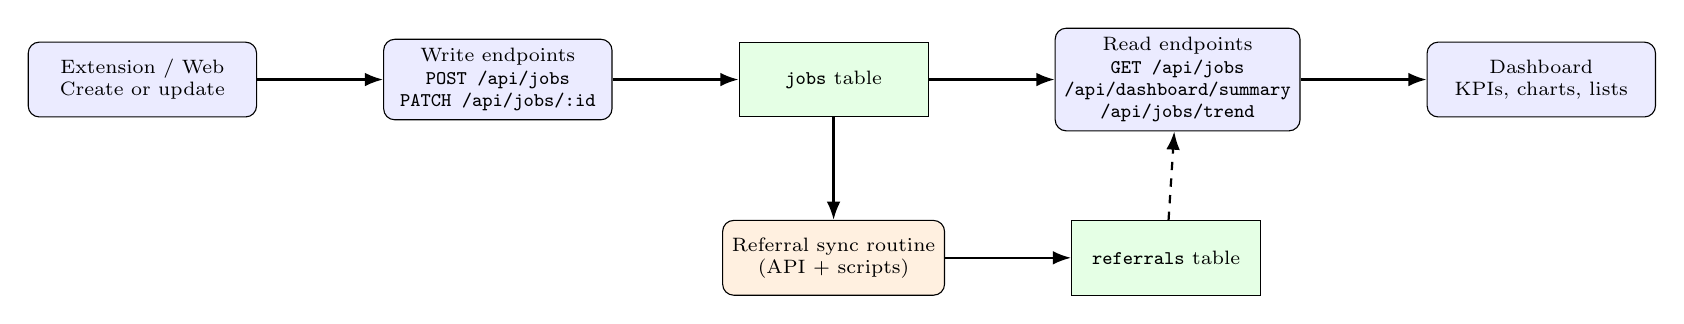
\begin{tikzpicture}[
  node distance=1.7cm and 1.6cm,
  every node/.style={font=\scriptsize},
  flowbox/.style={draw, rounded corners, align=center, minimum width=2.9cm, minimum height=0.95cm, fill=blue!8},
  store/.style={draw, align=center, minimum width=2.4cm, minimum height=0.95cm, fill=green!10},
  sync/.style={draw, rounded corners, align=center, minimum width=2.5cm, minimum height=0.95cm, fill=orange!12},
  edge/.style={-Latex, thick}
]
\node[flowbox] (source) {Extension / Web\\Create or update};
\node[flowbox, right=of source] (write) {Write endpoints\\\texttt{POST /api/jobs}\\\texttt{PATCH /api/jobs/:id}};
\node[store, right=of write] (jobs) {\texttt{jobs} table};
\node[flowbox, right=of jobs] (reads) {Read endpoints\\\texttt{GET /api/jobs}\\\texttt{/api/dashboard/summary}\\\texttt{/api/jobs/trend}};
\node[flowbox, right=of reads] (ui) {Dashboard\\KPIs, charts, lists};
\node[sync, below=1.3cm of jobs] (jobsync) {Referral sync routine\\(API + scripts)};
\node[store, right=of jobsync] (refs) {\texttt{referrals} table};

\draw[edge] (source) -- (write);
\draw[edge] (write) -- (jobs);
\draw[edge] (jobs) -- (reads);
\draw[edge] (reads) -- (ui);
\draw[edge] (jobs) -- (jobsync);
\draw[edge] (jobsync) -- (refs);
\draw[edge, dashed] (refs) -- (reads);
\end{tikzpicture}
\end{center}

\subsection{Referral Sync}
\begin{enumerate}[leftmargin=1.5em]
\item Referral rows are created directly via referral endpoints and indirectly via sync scripts.
\item Dashboard and referral trend endpoints consume aggregated counts.
\item \todoitem{Document source-of-truth rule when script and API both touch referral status.}
\end{enumerate}
\begin{center}
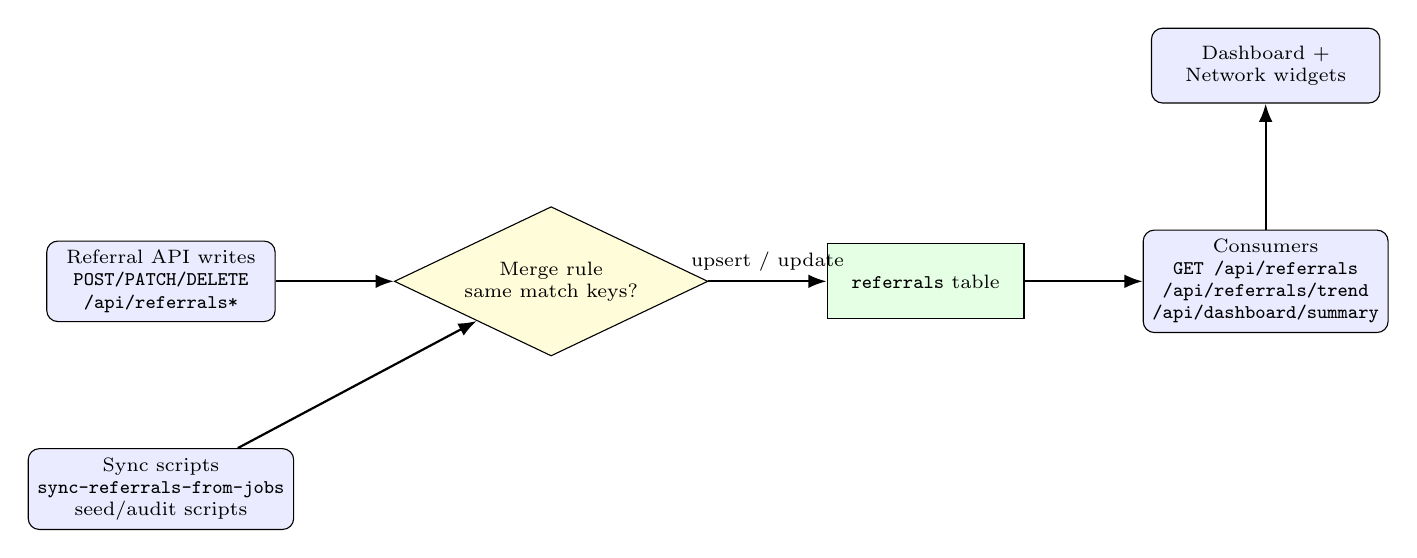
\begin{tikzpicture}[
  node distance=1.6cm and 1.5cm,
  every node/.style={font=\scriptsize},
  flowbox/.style={draw, rounded corners, align=center, minimum width=2.9cm, minimum height=0.95cm, fill=blue!8},
  store/.style={draw, align=center, minimum width=2.5cm, minimum height=0.95cm, fill=green!10},
  check/.style={draw, diamond, align=center, aspect=2.1, fill=yellow!15},
  edge/.style={-Latex, thick}
]
\node[flowbox] (apiwrite) {Referral API writes\\\texttt{POST/PATCH/DELETE}\\\texttt{/api/referrals*}};
\node[flowbox, below=of apiwrite] (scriptwrite) {Sync scripts\\\texttt{sync-referrals-from-jobs}\\seed/audit scripts};
\node[check, right=of apiwrite] (rule) {Merge rule\\same match keys?};
\node[store, right=of rule] (refstore) {\texttt{referrals} table};
\node[flowbox, right=of refstore] (consumers) {Consumers\\\texttt{GET /api/referrals}\\\texttt{/api/referrals/trend}\\\texttt{/api/dashboard/summary}};
\node[flowbox, above=of consumers] (ui2) {Dashboard +\\Network widgets};

\draw[edge] (apiwrite) -- (rule);
\draw[edge] (scriptwrite) -- (rule);
\draw[edge] (rule) -- node[above]{upsert / update} (refstore);
\draw[edge] (refstore) -- (consumers);
\draw[edge] (consumers) -- (ui2);
\end{tikzpicture}
\end{center}

\subsection{Friendship State Machine}
\begin{enumerate}[leftmargin=1.5em]
\item Request creation writes \texttt{friendships} with pending state.
\item Accept/reject/block transitions update state and timestamps.
\item Network dashboards read accepted relationships.
\item \todoitem{Confirm lock strategy prevents race updates and double transitions.}
\end{enumerate}
\begin{center}
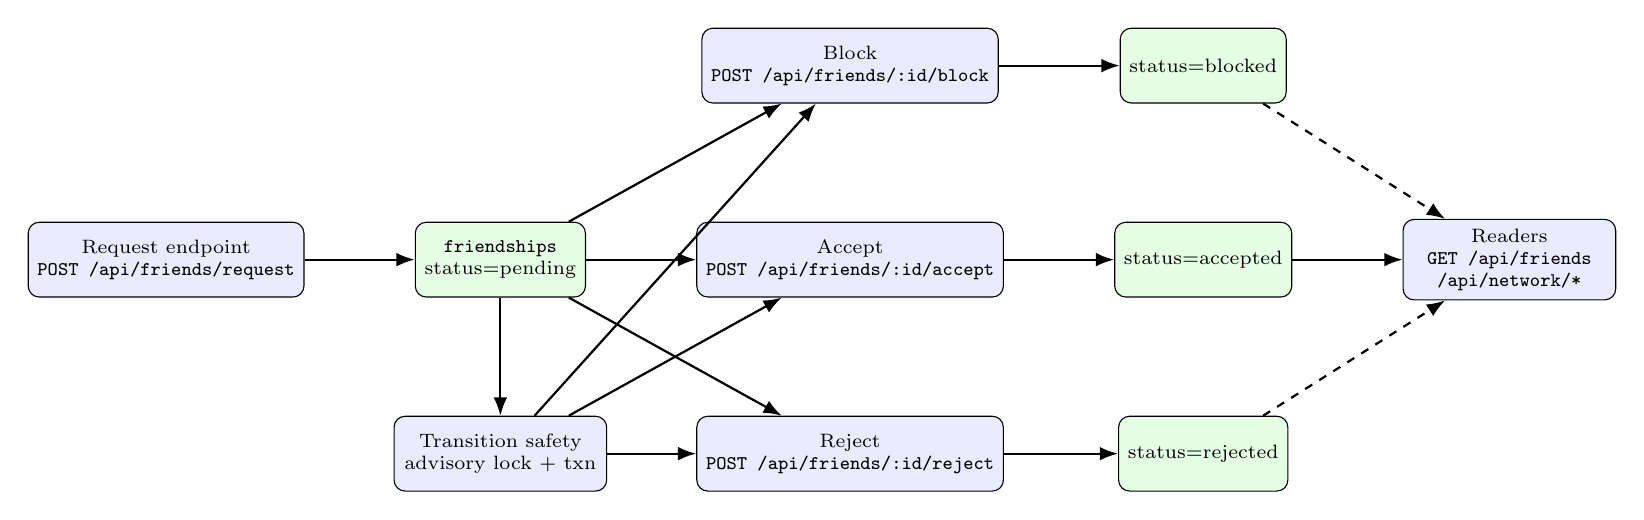
\begin{tikzpicture}[
  node distance=1.5cm and 1.4cm,
  every node/.style={font=\scriptsize},
  flowbox/.style={draw, rounded corners, align=center, minimum width=2.7cm, minimum height=0.95cm, fill=blue!8},
  state/.style={draw, rounded corners, align=center, minimum width=2.0cm, minimum height=0.95cm, fill=green!10},
  edge/.style={-Latex, thick}
]
\node[flowbox] (request) {Request endpoint\\\texttt{POST /api/friends/request}};
\node[state, right=of request] (pending) {\texttt{friendships}\\status=pending};
\node[flowbox, right=of pending] (accept) {Accept\\\texttt{POST /api/friends/:id/accept}};
\node[flowbox, below=of accept] (reject) {Reject\\\texttt{POST /api/friends/:id/reject}};
\node[flowbox, above=of accept] (block) {Block\\\texttt{POST /api/friends/:id/block}};
\node[state, right=of accept] (accepted) {status=accepted};
\node[state, below=of accepted] (rejected) {status=rejected};
\node[state, above=of accepted] (blocked) {status=blocked};
\node[flowbox, right=of accepted] (readers) {Readers\\\texttt{GET /api/friends}\\\texttt{/api/network/*}};
\node[flowbox, below=of pending] (lock) {Transition safety\\advisory lock + txn};

\draw[edge] (request) -- (pending);
\draw[edge] (pending) -- (accept);
\draw[edge] (pending) -- (reject);
\draw[edge] (pending) -- (block);
\draw[edge] (accept) -- (accepted);
\draw[edge] (reject) -- (rejected);
\draw[edge] (block) -- (blocked);
\draw[edge] (accepted) -- (readers);
\draw[edge, dashed] (rejected) -- (readers);
\draw[edge, dashed] (blocked) -- (readers);
\draw[edge] (pending) -- (lock);
\draw[edge] (lock) -- (accept);
\draw[edge] (lock) -- (reject);
\draw[edge] (lock) -- (block);
\end{tikzpicture}
\end{center}

\section{Release Checklist}
\begin{itemize}[leftmargin=1.5em]
\item Every DB call subsection has no remaining TODO lines.
\item Every write path has idempotency and conflict behavior documented.
\item Every aggregate query has index/perf review notes.
\item Every sync flow has staleness windows and refresh triggers documented.
\item Security review validates user scoping for every call.
\item Test coverage exists for all high-risk write and aggregate paths.
\end{itemize}

\end{document}
